% !TEX program = pdflatex
% Travail dirigé — ALM multi-étapes d'un fonds de pension canadien
% Compile avec pdflatex (ou xelatex : remplacer inputenc/fontenc/lmodern par fontspec)
\documentclass[11pt,letterpaper]{article}

\usepackage[utf8]{inputenc}
\usepackage[T1]{fontenc}
\usepackage[french]{babel}
\usepackage{lmodern}
\usepackage{amsmath,amssymb,amsthm}
\usepackage{booktabs}
\usepackage{graphicx}
\usepackage{geometry}
\geometry{margin=2.5cm}
\usepackage[colorlinks=true,linkcolor=black,citecolor=black,urlcolor=blue]{hyperref}
\usepackage{caption}

% ---------- Notation ----------
\newcommand{\E}{\mathbb{E}}
\newcommand{\prob}{\mathbb{P}}
\newcommand{\R}{\mathbb{R}}
\newcommand{\CSaR}{\mathrm{CSaR}}
\newcommand{\taustar}{\tau^{\star}}
\newcommand{\pos}[1]{\left(#1\right)^{+}}
\theoremstyle{definition}
\newtheorem{definition}{Définition}
\newtheorem{lemme}{Lemme}
\newtheorem{remarque}{Remarque}

\title{Gestion actif--passif d'un fonds de pension fermé\\
par programmation stochastique multi-étapes\\[0.5em]
\large Travail dirigé --- M.~Sc.\ Finance mathématique et computationnelle}
\author{Louckmane \textsc{Alma Mousbahou}\\[0.3em]
\small Université de Montréal --- Département de mathématiques et de statistique\\
\small Sous la direction du Pr Fabian \textsc{Bastin}}
\date{\today}

\begin{document}
\maketitle

\begin{abstract}
Nous étudions le problème de gestion actif--passif (ALM) d'un fonds de pension à
prestations déterminées \emph{fermé}, pour lequel l'allocation d'actifs constitue le
seul levier de pilotage. Le problème est formulé comme un programme linéaire de recours
multi-étapes sur arbre de scénarios, combinant un objectif terminal fondé sur le
\emph{Conditional Surplus-at-Risk} (CSaR) et des contraintes de solvabilité
intermédiaires de type \emph{Integrated Chance Constraints} (ICC). Le modèle est
calibré sur cinq FNB canadiens et résolu en Julia (JuMP/HiGHS). Nous introduisons un
plancher de faisabilité $\taustar$ --- la plus petite tolérance de manque uniforme
atteignable --- qui sert à la fois d'ancrage robuste pour la calibration des
contraintes et de mesure du coût de solvabilité d'un régime fermé. L'évaluation hors
échantillon en horizon roulant et les analyses de sensibilité quantifient la valeur de
la flexibilité multi-étapes et la dépendance des résultats à la fenêtre d'estimation
des rendements espérés.
\end{abstract}

\tableofcontents
\newpage

% ==================================================================
\section{Introduction}
% ==================================================================

La gestion actif--passif (\emph{asset-liability management}, ALM) d'un fonds de
pension à prestations déterminées consiste à piloter conjointement un portefeuille
d'actifs et un passif actuariel, de sorte que le fonds honore ses engagements envers
les participants tout en maîtrisant le risque de sous-financement. Lorsque le régime
est \emph{ouvert}, le promoteur dispose de plusieurs leviers~: la politique de
placement, bien sûr, mais aussi les cotisations régulières et, en cas de dégradation
du ratio de capitalisation, des cotisations de redressement. La littérature
institutionnelle, notamment le modèle développé pour les fonds néerlandais par
Klein~Haneveld, Streutker et van~der~Vlerk~\cite{KHSV2010}, traite précisément de
l'arbitrage entre ces leviers~: l'objectif y est de minimiser le coût de financement
sous contraintes de solvabilité.

Le présent travail considère la situation, plus contrainte, d'un fonds
\emph{fermé}~: aucun nouveau participant, aucune cotisation après la dotation
initiale. Ce cas n'est pas une simple curiosité académique --- il correspond aux
régimes en extinction (\emph{run-off}), fréquents lorsque des employeurs ferment
leur régime à prestations déterminées et laissent le passif existant s'éteindre par
le versement graduel des rentes. Dans cette configuration, l'allocation d'actifs
devient le \emph{seul} levier de gestion~: le fonds doit financer un flux de
décaissements exogène et contenir son risque de sous-financement uniquement par la
composition de son portefeuille, révisée au fil de l'information disponible. La
question centrale est alors double~: quelle allocation dynamique adopter, et ---
plus fondamentalement --- quel niveau de solvabilité est-il seulement
\emph{possible} de garantir sans l'appui de cotisations~?

Pour y répondre, nous formulons le problème comme un programme de recours
multi-étapes sur arbre de scénarios, dans le cadre de la programmation stochastique
linéaire~\cite{KHvdVR2020}. L'incertitude porte conjointement sur les rendements de
cinq classes d'actifs négociables au Canada --- actions canadiennes et américaines,
obligations nominales de long terme, obligations à rendement réel, et or comme
diversificateur satellite --- et sur la croissance du passif actuariel. À chaque
n\oe ud de l'arbre, le gestionnaire réalloue le portefeuille sans connaître l'avenir
(non-anticipativité), après avoir servi le décaissement de la période. Deux objets du
chapitre~6 de~\cite{KHvdVR2020} structurent la gestion du risque. D'une part,
l'objectif terminal pénalise le \emph{Conditional Surplus-at-Risk}
$\CSaR_\gamma(S_T)$ du surplus final $S_T = A_T - L_T$, c'est-à-dire l'espérance de
la pire fraction $(1-\gamma)$ des surplus~; sa forme variationnelle
(lemme~6.4.2 de~\cite{KHvdVR2020}, dans l'esprit de
Rockafellar--Uryasev~\cite{RU2000}) en permet une linéarisation exacte. D'autre
part, des \emph{Integrated Chance Constraints} bornent, à chaque période
intermédiaire, le manque espéré $\E[\pos{L_t - A_t}]$ en proportion du passif~: là où
une contrainte en probabilité rendrait le problème non convexe, l'ICC préserve la
linéarité tout en contrôlant à la fois la fréquence \emph{et} la profondeur des
déficits.

La calibration de la tolérance $\delta$ de ces contraintes s'est révélée être un
enjeu à part entière, et constitue l'un des apports méthodologiques de ce travail.
Un seuil fixé arbitrairement expose à l'infaisabilité~: le profil de manque d'un
fonds fermé est élevé, et sensible à la fenêtre d'estimation des paramètres. Nous
ancrons donc $\delta$ à un \emph{plancher de faisabilité} $\taustar$, défini comme
la plus petite tolérance uniforme atteignable et calculé par un programme minimax
auxiliaire. Ce plancher garantit la faisabilité par construction, rend la
calibration robuste à toute mise à jour des données et --- surtout --- possède une
interprétation économique propre~: $\taustar$ mesure le niveau de solvabilité
incompressible d'un fonds fermé. Sa variante \emph{conditionnelle}, qui exige la
tenue du seuil état par état plutôt qu'en espérance vue de la racine, s'avère
beaucoup plus exigeante~; l'écart entre les deux chiffre le prix de la cohérence
temporelle et, en creux, la valeur des cotisations de redressement dont le fonds
fermé est privé.

Le modèle est implémenté en Julia (JuMP, solveur HiGHS) et calibré sur les cours
ajustés mensuels de cinq FNB cotés à la Bourse de Toronto. Le dispositif
expérimental comporte trois volets~: une \emph{validation} de la mécanique
(confrontation de la CSaR optimisée à sa forme fermée gaussienne dans un cas à une
période~; stabilité de la décision initiale entre réalisations de l'arbre)~; une
\emph{évaluation hors échantillon} en horizon roulant, où la politique optimisée ---
re-résolue à chaque date depuis l'état courant --- est comparée à des portefeuilles
à poids fixes sur des trajectoires simulées indépendantes~; et des \emph{analyses de
sensibilité} portant sur l'aversion au risque, la tolérance de solvabilité, la
capitalisation initiale, le rythme de décaissement et, de façon critique, les
rendements espérés. Ce dernier point mérite d'être souligné dès l'introduction~: la
fenêtre d'estimation disponible (2013--2026) correspond à un marché haussier
exceptionnel pour les actions, et les moyennes estimées en héritent un optimisme
qu'aucune covariance ne compense. Plutôt que de dissimuler cette fragilité, nous la
quantifions~: une part substantielle de la sécurité apparente du fonds est
\emph{empruntée} à cette fenêtre, et nous mesurons combien.

Le périmètre du travail est volontairement resserré. Le passif est exogène et
indépendant des rendements~; la mesure de risque terminale est statique~; les
rendements sont log-normaux i.i.d.~; la poche d'actions américaines est portée
non couverte, le risque de change étant ainsi modélisé implicitement dans les
rendements en dollars canadiens. Ces
hypothèses, discutées en section~\ref{sec:limites}, préservent la linéarité et la
lisibilité du prototype~; leurs relâchements naturels --- cotisations, couplage
taux--passif, mesures de risque imbriquées --- sont esquissés comme extensions.

La suite du document est organisée comme suit. La section~\ref{sec:contexte}
rappelle les mécanismes d'un régime à prestations déterminées et situe le
travail dans la littérature de l'ALM par programmation stochastique. La
section~\ref{sec:cadre} rappelle
le cadre des modèles de recours et les définitions de l'ICC et de la CSaR. La
section~\ref{sec:modele} formule le programme linéaire complet et introduit le
plancher $\taustar$. La section~\ref{sec:donnees} décrit les données, l'univers
d'actifs et la génération de l'arbre. La section~\ref{sec:implementation} présente
l'implémentation et les tests de validation. La section~\ref{sec:resultats} expose
les résultats~: cas de base, comparaison hors échantillon et analyses économiques.
La section~\ref{sec:limites} discute les limites et les extensions, et la
section~\ref{sec:conclusion} conclut.

% ==================================================================
\section{Fonds de pension à prestations déterminées~: mécanismes et
littérature}\label{sec:contexte}
% ==================================================================

Avant d'entrer dans le formalisme, cette section situe le travail~: d'abord en
rappelant les mécanismes économiques d'un fonds de pension à prestations
déterminées --- ce qui précise de quels leviers le gestionnaire dispose, et
lesquels disparaissent quand le régime ferme ---, ensuite en parcourant la
littérature de l'ALM par programmation stochastique dont notre modèle est
l'héritier direct.

\subsection{Mécanismes d'un régime à prestations déterminées}
\label{ssec:mecanismes}

Dans un régime à \emph{prestations déterminées} (PD), le promoteur promet aux
participants une rente définie par une formule contractuelle --- typiquement un
pourcentage du salaire de référence par année de service --- versée de la
retraite au décès. C'est le trait distinctif du PD~: le \emph{montant} de la
prestation est garanti, et c'est donc le promoteur, non le participant, qui
porte les risques de placement et de longévité~; dans un régime à cotisations
déterminées (CD), la logique est inverse~\cite{Broadbent2006}.

La contrepartie comptable de cette promesse est le \emph{passif actuariel}
$L$~: la valeur actualisée des prestations futures associées aux droits déjà
acquis, calculée à partir de tables de mortalité et d'un taux d'actualisation
prescrit ou dérivé des marchés. Ce passif est une grandeur sensible~: il
s'accroît de l'intérêt sur les droits (l'actualisation « déroule » à mesure que
les paiements se rapprochent), des droits nouveaux si le régime est ouvert, et
des revalorisations~; il décroît des prestations versées. Le rapport entre
l'actif et ce passif, le \emph{ratio de capitalisation} $\mathrm{FR} = A/L$,
est la boussole de la gestion comme de la surveillance réglementaire~: la
plupart des juridictions --- dont le cadre canadien, avec ses évaluations
actuarielles périodiques, et le cadre néerlandais qui a motivé la littérature
dont nous nous inspirons --- imposent des exigences de capitalisation et,
lorsque $\mathrm{FR}$ passe sous un seuil, un \emph{plan de redressement} à
horizon défini~\cite{KHSV2010}.

Le gestionnaire d'un régime \emph{ouvert} dispose pour cela de trois familles
de leviers~: la politique de placement~; les cotisations régulières, dont le
taux peut être ajusté~; et les mesures exceptionnelles --- cotisations de
redressement du promoteur et, dans certaines juridictions comme les Pays-Bas,
indexation conditionnelle voire réduction des droits en dernier
recours~\cite{KHSV2010}. Or la tendance structurelle des
dernières décennies est à la fermeture de ces régimes~: sous l'effet du coût,
de la volatilité comptable et du transfert de risque vers les employeurs, une
grande partie des promoteurs privés ont fermé leur régime PD aux nouveaux
entrants, puis gelé l'accumulation de droits, au profit de régimes
CD~\cite{Broadbent2006}. Le régime devient alors \emph{fermé}, en extinction
(\emph{run-off})~: le stock de droits existant s'éteint par le versement
graduel des rentes, sans flux entrant pour le renouveler. Deux issues
s'offrent au promoteur~: transférer le passif à un assureur (rachat,
\emph{buy-out}) --- au prix d'une prime --- ou gérer l'extinction en interne.
C'est ce second cas qui nous occupe~: les leviers de cotisation ont disparu,
l'horizon est fini, les décaissements nets croissent relativement au passif
résiduel, et la politique de placement est le seul instrument restant. La
question quantitative centrale --- quel niveau de solvabilité l'allocation
seule peut-elle garantir~? --- est précisément celle que le plancher
$\taustar$ de la section~\ref{ssec:taustar} formalisera.

\subsection{Revue de littérature}\label{ssec:revue}

\paragraph{L'ALM par programmation stochastique et la lignée des ICC.}
Formuler la gestion actif--passif comme un programme stochastique multi-étapes
sur arbre de scénarios est une approche établie depuis les années~1980, dont
l'attrait tient à ce qu'elle épouse la réalité institutionnelle~: décisions
datées et révisables, contraintes réglementaires et de politique de placement
imposées explicitement, et --- sur support fini --- réduction à un programme
linéaire de grande taille~\cite[chap.~1--3]{KHvdVR2020}. Pour les fonds de
pension, la lignée directement pertinente pour notre travail est celle qui
s'est développée autour des fonds néerlandais, et son intérêt pour nous tient
moins à sa chronologie qu'à un arbitrage technique qu'elle a explicitement
tranché.

Dert~\cite{Dert1995} formule le premier modèle multi-étapes de fonds de
pension dont les contraintes de solvabilité sont des contraintes \emph{en
probabilité}~: exiger $\prob(A_t \ge L_t) \ge 1-\alpha$ à chaque période.
Cette écriture est intuitive et proche du langage réglementaire, mais elle
coûte cher~: sur support fini, elle impose de sélectionner les scénarios en
défaut, donc des variables binaires, et le problème devient un programme en
nombres entiers mixtes --- voie que Drijver~\cite{Drijver2005} poursuit et
étend aux décisions discrètes du promoteur. Klein~Haneveld, Streutker et
van~der~Vlerk~\cite{KHSV2010}, notre référence principale, opèrent le
basculement qui nous intéresse~: remplacer ces contraintes en probabilité par
des contraintes de manque \emph{intégrées} (ICC), instrument introduit par
Klein~Haneveld~\cite{KH1986}. Le gain est double, et les deux volets comptent
pour nous. Économiquement, l'ICC contrôle la \emph{profondeur} des déficits et
pas seulement leur fréquence --- distinction pertinente pour un fonds fermé,
dont le risque n'est pas tant de passer sous la barre que d'y descendre
loin. Techniquement, la convexité est préservée et le programme reste
linéaire, ce qui autorise l'exploration systématique de la tolérance dont ce
travail fait son objet central (section~\ref{ssec:implementation-code}).

\paragraph{Mesure du risque terminal.}
Le second ingrédient de notre objectif s'inscrit dans la littérature des
mesures de risque cohérentes d'Artzner, Delbaen, Eber et
Heath~\cite{Artzner1999}~: la CVaR y satisfait les axiomes que le quantile
viole, et surtout, la représentation variationnelle de Rockafellar et
Uryasev~\cite{RU2000} la rend linéarisable exactement sur support fini. Le
\emph{Conditional Surplus-at-Risk} du chapitre~6 de~\cite{KHvdVR2020} en est
la transposition au surplus d'un bilan. Notre montage --- CSaR terminale dans
l'objectif, ICC en contraintes de chemin --- suit ce chapitre en confiant
risque terminal et risque de trajectoire à deux instruments distincts, tous
deux compatibles avec la programmation linéaire~; c'est cette compatibilité,
plus que l'élégance de chacun pris isolément, qui fait la cohérence du
dispositif.

\paragraph{Positionnement.}
Deux autres traditions traitent le même problème et éclairent, par contraste,
le choix de la nôtre. L'optimisation de surplus à une période, issue de Sharpe
et Tint~\cite{SharpeTint1990}, prolonge Markowitz au bilan complet et fonde la
pratique du \emph{liability-driven investment}~: elle capture l'appariement
actif--passif, mais ni la dynamique de recours ni les contraintes de chemin.
À l'autre extrême, le contrôle stochastique en temps continu produit des
politiques analytiques élégantes mais s'accommode mal des bornes de placement
et des seuils réglementaires qui font le quotidien d'un fonds réel. La
programmation stochastique occupe l'entre-deux~: moins élégante, mais capable
d'imposer exactement les contraintes institutionnelles --- critère décisif
ici, puisque notre question porte précisément sur ce qu'une politique
\emph{contrainte} peut garantir.

Reste l'écart que ce travail vise à combler. Tous les modèles de la lignée
néerlandaise supposent disponible le levier des cotisations~: c'est même leur
objet, puisqu'ils arbitrent entre placement et financement pour minimiser le
coût du second. Le fonds \emph{fermé}, où ce levier a disparu et où
l'allocation est le seul recours, est peu traité pour lui-même --- alors que
la fermeture des régimes PD en fait une situation de plus en plus
courante~\cite{Broadbent2006}. Or cette absence n'est pas un cas particulier
anodin~: elle force l'affaiblissement des ICC conditionnelles en ICC
inconditionnelles (section~\ref{ssec:positionnement}) et fait émerger la
question de faisabilité --- quel seuil de solvabilité est seulement
\emph{atteignable}~? --- que le plancher $\taustar$
(section~\ref{ssec:taustar}) formalise et mesure. C'est le pont que nous
proposons entre le modèle institutionnel de~\cite{KHSV2010} et le régime en
extinction.

% ==================================================================
\section{Cadre théorique}\label{sec:cadre}
% ==================================================================

Cette section rassemble les outils de programmation stochastique sur lesquels
repose la formulation~: les modèles de recours multi-étapes sur arbre de scénarios,
puis les deux instruments de gestion du risque empruntés au chapitre~6
de~\cite{KHvdVR2020} --- les contraintes de manque intégrées et le
\emph{Conditional Surplus-at-Risk}. Nous terminons en situant notre cas d'étude par
rapport au modèle institutionnel dont il est une version épurée.

\subsection{Modèles de recours multi-étapes}\label{ssec:recours}

Un problème de décision séquentielle sous incertitude alterne décisions et
observations~: le décideur choisit une première action, observe une réalisation
aléatoire, ajuste sa décision, observe à nouveau, et ainsi de suite jusqu'à
l'horizon $T$. Les modèles de recours~\cite[chap.~1--3]{KHvdVR2020} formalisent
cette alternance en exigeant que chaque décision ne dépende que de l'information
disponible au moment où elle est prise --- c'est la contrainte de
\emph{non-anticipativité}.

Lorsque le processus stochastique sous-jacent est approché par un support fini, la
structure d'information se représente par un \emph{arbre de scénarios}. Chaque
n\oe ud $n$ de l'arbre correspond à une histoire partielle du processus jusqu'à la
période $t(n)$~; son parent est noté $a(n)$, sa probabilité (inconditionnelle)
$p_n$, et l'ensemble des feuilles --- les n\oe uds terminaux, identifiés aux
scénarios complets --- est noté $\mathcal F$. Un scénario est ainsi un chemin de la
racine à une feuille, et deux scénarios qui partagent leur histoire jusqu'à la
période $t$ passent par les mêmes n\oe uds jusqu'à $t$.

La non-anticipativité admet alors une formulation dite \emph{structurelle}~: il
suffit d'indexer les variables de décision par les n\oe uds plutôt que par les
scénarios. Une décision $x_n$ attachée au n\oe ud $n$ est par construction commune à
tous les scénarios passant par $n$, puisqu'ils sont indistinguables à cette date.
Cette représentation évite d'introduire les contraintes d'égalité explicites
($x^s = x^{s'}$ pour tous scénarios $s, s'$ indistinguables à la date $t$) qu'exige
la formulation par scénarios, et réduit d'autant la taille du programme. C'est elle
que nous adoptons.

Sur un arbre fini, un problème de recours multi-étapes dont les coûts et les
contraintes sont linéaires en les décisions se réduit à un unique programme
linéaire déterministe de grande taille --- dit \emph{équivalent déterministe} ---
dont les variables sont l'ensemble des décisions indexées par les n\oe uds. C'est
cette propriété qui rend l'approche opérationnelle~: la difficulté conceptuelle
(décider sous information partielle) est absorbée par la structure de l'arbre, et
la difficulté calculatoire se ramène à la résolution d'un programme linéaire, pour
laquelle des solveurs performants existent. La contrepartie est la croissance
exponentielle du nombre de n\oe uds avec l'horizon, qui contraint en pratique le
branchement et la profondeur de l'arbre~; nous y revenons en
section~\ref{sec:donnees}.

\subsection{Contraintes de manque intégrées (ICC)}\label{ssec:icc}

Soit $A$ l'actif d'un fonds et $L$ son passif à une date donnée, tous deux
aléatoires. La manière la plus naturelle d'exiger la solvabilité est une
\emph{contrainte en probabilité} (\emph{chance constraint})~:
$\prob(A \ge L) \ge 1 - \alpha$. Elle souffre de deux défauts bien connus. D'abord,
elle détruit en général la convexité du problème~: sur un support fini, elle
équivaut à sélectionner les scénarios en défaut, ce qui introduit une combinatoire
(variables binaires). Ensuite, elle est aveugle à la \emph{profondeur} du
déficit~: un scénario où l'actif manque d'un dollar et un scénario où il manque de
la moitié du passif pèsent identiquement.

Les \emph{contraintes de manque intégrées} (\emph{Integrated Chance Constraints},
ICC), introduites par Klein Haneveld~\cite{KH1986} et étudiées à la
section~6.5 de~\cite{KHvdVR2020}, corrigent ces deux défauts en
contraignant non la probabilité du déficit mais son \emph{espérance}~:
\begin{equation}\label{eq:icc-generique}
\E\!\left[\pos{L - A}\right] \;\le\; \delta \cdot \E[L],
\end{equation}
où $\delta \ge 0$ est une tolérance exprimée en proportion du passif espéré, et
$\pos{y} = \max(y, 0)$. Le membre de gauche, appelé \emph{manque espéré}
(\emph{expected shortfall} au sens du livre), intègre à la fois la fréquence et la
sévérité des états de déficit. Surtout, la fonction
$(A) \mapsto \E[\pos{L - A}]$ est convexe, et sur un support fini la
contrainte~\eqref{eq:icc-generique} se linéarise exactement à l'aide de variables
auxiliaires~: en introduisant $D_n \ge L_n - A_n$, $D_n \ge 0$ pour chaque n\oe ud
$n$ concerné, la contrainte devient $\sum_n p_n D_n \le \delta \sum_n p_n L_n$.
Comme $D_n$ n'apparaît que dans des contraintes qui la poussent vers le bas, toute
solution optimale peut être prise avec $D_n = \pos{L_n - A_n}$~: la linéarisation
est sans perte.

L'ICC conserve donc la linéarité du programme --- aucune variable binaire --- tout
en fournissant un contrôle économiquement plus riche que la contrainte en
probabilité. Son paramètre $\delta$ s'interprète directement~: c'est le déficit
moyen maximal toléré, en cents par dollar de passif. Enfin, le multiplicateur
optimal (dual) associé à~\eqref{eq:icc-generique} mesure le coût marginal de la
solvabilité~: de combien l'objectif s'améliorerait si l'on relâchait la tolérance
d'une unité. Nous exploiterons systématiquement cette lecture.

\subsection{Conditional Surplus-at-Risk et linéarisation}\label{ssec:csar}

L'ICC contrôle le chemin~; il reste à choisir un critère pour l'état terminal.
Suivant la section~6.4 de~\cite{KHvdVR2020}, nous retenons le
\emph{Conditional Surplus-at-Risk} du surplus terminal, qui est à la maximisation
du surplus ce que la CVaR de Rockafellar--Uryasev~\cite{RU2000} est à la
minimisation des pertes.

\begin{definition}[CSaR, d'après la définition 6.4.1 de \cite{KHvdVR2020}]
Soit $S$ une variable aléatoire de surplus et $\gamma \in (0,1)$ un niveau de
confiance. Le \emph{Conditional Surplus-at-Risk} de niveau $\gamma$, noté
$\CSaR_\gamma(S)$, est l'espérance de $S$ conditionnelle à sa pire queue de masse
$1-\gamma$. Sur une distribution discrète, la queue est complétée au prorata de la
masse manquante lorsque le quantile tombe à l'intérieur d'un atome.
\end{definition}

Contrairement à un quantile (Surplus-at-Risk), la CSaR regarde \emph{au-delà} du
quantile~: elle moyenne tout ce qui se passe dans la queue basse, et pénalise donc
la profondeur des mauvais scénarios, en cohérence avec le choix de l'ICC pour le
chemin --- et avec les exigences de cohérence dégagées par la littérature des
mesures de risque~\cite{Artzner1999}. C'est par ailleurs une fonctionnelle concave de la distribution du surplus,
propriété qui fonde le résultat suivant.

\begin{lemme}[forme variationnelle, lemme 6.4.2 de \cite{KHvdVR2020}]
\label{lem:csar-var}
Pour tout $\gamma \in (0,1)$,
\begin{equation}\label{eq:csar-var}
\CSaR_\gamma(S) \;=\; \max_{\eta \in \R}\;
\left\{\, \eta \;-\; \frac{1}{1-\gamma}\, \E\!\left[\pos{\eta - S}\right] \right\},
\end{equation}
le maximum étant atteint en $\eta^\star$ égal au quantile de niveau $1-\gamma$ de
$S$.
\end{lemme}

La représentation~\eqref{eq:csar-var} est l'analogue exact de la formule de
Rockafellar--Uryasev pour la CVaR, transposée du côté \og surplus \fg. Son intérêt
opérationnel est immédiat~: sur un support fini $\{S_n, p_n\}_{n \in \mathcal F}$,
le terme $\E[\pos{\eta - S}]$ se linéarise par des variables $u_n \ge \eta - S_n$,
$u_n \ge 0$, de sorte que
\begin{equation}\label{eq:csar-lp}
\CSaR_\gamma(S) \;=\; \max_{\eta,\, u \ge 0}\;
\Big\{\, \eta - \tfrac{1}{1-\gamma} \textstyle\sum_{n \in \mathcal F} p_n u_n
\;:\; u_n \ge \eta - S_n \Big\}.
\end{equation}
Lorsque cette expression apparaît, affectée d'un poids strictement positif, dans un
objectif que l'on maximise (ou avec le signe opposé dans un objectif que l'on
minimise), l'optimisation pousse chaque $u_n$ sur sa borne
$\pos{\eta - S_n}$ et $\eta$ sur le quantile~: la relaxation est exacte, et la CSaR
s'optimise \emph{conjointement} avec les décisions de portefeuille dans un même
programme linéaire.

\begin{remarque}\label{rem:lambda-zero}
L'exactitude requiert un poids strictement positif sur la CSaR dans l'objectif. Si
ce poids est nul, les variables $(\eta, u)$ deviennent indéterminées et la valeur
\og CSaR \fg{} lue dans le programme n'a pas de sens~; il faut alors la recalculer
ex post à partir de la distribution du surplus. Ce point, anodin en apparence,
concerne concrètement l'analyse de sensibilité au poids de risque
(section~\ref{sec:resultats}).
\end{remarque}

\subsection{Positionnement~: le modèle institutionnel et le cas fermé}
\label{ssec:positionnement}

Le modèle ALM de référence pour notre travail est celui développé par
Klein~Haneveld, Streutker et van~der~Vlerk~\cite{KHSV2010} pour les fonds de
pension néerlandais. Il s'agit d'un modèle de recours multi-étapes dans lequel le
promoteur dispose de cotisations régulières et de cotisations de redressement~;
l'objectif minimise le coût de financement (niveau et variabilité des cotisations),
et la solvabilité est imposée par des ICC \emph{conditionnelles}, écrites n\oe ud
par n\oe ud~: à chaque état de l'arbre, le manque espéré des états successeurs
immédiats est borné. Cette écriture conditionnelle donne au gestionnaire une
garantie de cohérence temporelle --- le seuil vaut dans \emph{chaque} état, pas
seulement en moyenne vue de la racine --- et le levier des cotisations la rend
atteignable.

Notre cas d'étude s'obtient en fermant le fonds~: cotisations nulles après la
dotation initiale, passif en extinction, allocation comme seul recours. Deux
conséquences structurent la formulation de la section~\ref{sec:modele}. D'une part,
l'objectif change de nature~: sans cotisations à minimiser, le critère se reporte
sur le surplus terminal, dont nous maximisons un compromis
espérance--CSaR. D'autre part, l'exigence de solvabilité doit être affaiblie
d'ICC conditionnelles en ICC \emph{inconditionnelles} (par période, vues de la
racine)~: privé du levier des cotisations, le fonds fermé ne peut simplement pas
garantir un seuil serré état par état. Cette impossibilité n'est pas une conjecture~;
nous la quantifierons précisément à l'aide du plancher de faisabilité conditionnel
(sections~\ref{ssec:taustar} et~\ref{sec:resultats}), et l'écart entre les deux
planchers mesurera ce que la fermeture du fonds coûte en capacité de solvabilité.

% ==================================================================
\section{Formulation du modèle}\label{sec:modele}
% ==================================================================

Nous formulons maintenant le programme complet. Les paramètres et la calibration
numérique sont décrits en section~\ref{sec:donnees}~; ici, l'arbre
$\{p_n, r_n, L_n\}$ est donné.

\subsection{Dynamique de l'actif et du passif}\label{ssec:dynamique}

L'horizon est découpé en $T$ périodes, une période représentant une année~: les
paramètres annualisés de la section~\ref{sec:donnees} sont tirés une fois par
période, et l'horizon effectif est donc de $T = 5$~ans. L'arbre de scénarios
porte, à chaque n\oe ud
$n$ de profondeur $t(n) \ge 1$, un vecteur de rendements simples
$r_n \in \R^{N_a}$ réalisés entre $t(n)-1$ et $t(n)$, et une valeur de passif
$L_n$. Le passif évolue de façon exogène,
$L_n = L_{a(n)} (1 + g_n)$, où $g_n$ est un taux de croissance actuariel tiré
indépendamment des rendements~; $L_n$ représente la valeur actualisée des
prestations restantes dans l'état $n$.

Le fonds sert à chaque période un décaissement net exogène
\begin{equation}\label{eq:decaissement}
F_t \;=\; \varphi_t \,\E[L_t], \qquad t = 0, \dots, T-1,
\end{equation}
où le profil $(\varphi_t)$ est croissant~: la charge de prestations s'alourdit
relativement au passif à mesure que le régime s'éteint. Le choix d'un décaissement
déterministe (proportionnel au passif \emph{espéré} plutôt qu'au passif réalisé)
maintient la séparation entre l'aléa et les flux et simplifie la lecture~; il est
discuté en section~\ref{sec:limites}.

Au n\oe ud $n$ non terminal, l'actif disponible $A_n$ sert d'abord le décaissement
$F_{t(n)}$, puis le solde investissable
\begin{equation}\label{eq:investissable}
I_n \;=\; A_n - F_{t(n)}
\end{equation}
est réparti entre les $N_a$ actifs~: $x_{n,i} \ge 0$ désigne le \emph{montant}
investi dans l'actif $i$. L'actif du n\oe ud suivant s'en déduit,
\begin{equation}\label{eq:propagation}
A_m \;=\; \sum_{i=1}^{N_a} x_{n,i}\,(1 + r_{m,i})
\qquad \text{pour tout enfant } m \text{ de } n,
\end{equation}
avec $A_{\text{racine}} = A_0$ donné. Le \emph{surplus} d'un n\oe ud est
$S_n = A_n - L_n$~; le \emph{ratio de capitalisation} est $A_n / L_n$. Aucun
emprunt ni vente à découvert n'est permis, et la politique de placement impose des
bornes proportionnelles
\begin{equation}\label{eq:bornes}
\underline w_i\, I_n \;\le\; x_{n,i} \;\le\; \overline w_i\, I_n,
\qquad i = 1, \dots, N_a,
\end{equation}
qui restent linéaires puisque $I_n$ est une variable du programme. On notera
qu'avec $x_{n,i} \ge 0$ et la contrainte de
budget~\eqref{eq:c-budget}, la faisabilité impose implicitement
$A_n \ge F_{t(n)}$ à chaque n\oe ud de décision --- le fonds doit pouvoir payer
le décaissement de la période~; cette contrainte de capacité de paiement fait
partie du modèle, même si elle ne se révèle jamais liante sur les arbres que
nous générons. Les frais de
transaction ne sont pas modélisés.

\subsection{Le programme linéaire de recours}\label{ssec:lp}

Les variables sont les montants $x_{n,i}$ (n\oe uds non terminaux), les actifs
$A_n$, les déficits $D_n$, et les variables de linéarisation de la CSaR
$(\eta, u_n)$ sur les feuilles. Avec $\gamma \in (0,1)$ le niveau de confiance et
$\lambda > 0$ le poids d'aversion au risque, le programme s'écrit
\begin{align}
\min_{x,\,A,\,D,\,\eta,\,u}\quad
& -\sum_{n \in \mathcal F} p_n (A_n - L_n)
\;-\; \lambda \Big( \eta - \tfrac{1}{1-\gamma}
      \sum_{n \in \mathcal F} p_n u_n \Big)
\label{eq:objectif}\\[2pt]
\text{s.c.}\quad
& A_{\text{racine}} = A_0, \qquad
A_m = \textstyle\sum_i x_{a(m),i} (1 + r_{m,i}), \quad m \ne \text{racine},
\label{eq:c-prop}\\
& \textstyle\sum_i x_{n,i} = A_n - F_{t(n)}, \qquad n \notin \mathcal F,
\label{eq:c-budget}\\
& \underline w_i (A_n - F_{t(n)}) \le x_{n,i} \le \overline w_i (A_n - F_{t(n)}),
\qquad n \notin \mathcal F,\ i = 1,\dots,N_a,
\label{eq:c-bornes}\\
& D_n \ge L_n - A_n, \qquad D_n \ge 0, \qquad \text{tout } n,
\label{eq:c-deficit}\\
& u_n \ge \eta - (A_n - L_n), \qquad u_n \ge 0, \qquad n \in \mathcal F,
\label{eq:c-u}\\
& \sum_{n\,:\,t(n) = t} p_n D_n \;\le\; \delta_t\, \E[L_t],
\qquad t = 1, \dots, T-1.
\label{eq:c-icc}
\end{align}
L'objectif~\eqref{eq:objectif} maximise le compromis
$\E[S_T] + \lambda\,\CSaR_\gamma(S_T)$~; par le
lemme~\ref{lem:csar-var} et la remarque qui le suit, la valeur optimale du bloc
$(\eta, u)$ coïncide exactement avec la CSaR du surplus terminal dès que
$\lambda > 0$. Les contraintes~\eqref{eq:c-prop}--\eqref{eq:c-bornes} portent la
dynamique et la politique de placement~; la non-anticipativité est structurelle
(les $x_n$ sont indexés par n\oe ud). La contrainte~\eqref{eq:c-deficit} définit le
déficit linéarisé, et~\eqref{eq:c-icc} est l'ICC inconditionnelle de la période $t$.

Trois choix de conception méritent d'être explicités. \emph{Premièrement}, risque
terminal et risque de chemin sont confiés à deux instruments distincts~: la CSaR
gouverne la queue de $S_T$ dans l'objectif, les ICC gardent les périodes
intermédiaires $t = 1, \dots, T-1$ en contrainte. La période terminale est exclue
des ICC --- l'y inclure reviendrait à contraindre deux fois la même tranche de
risque, en conflit avec l'objectif~; la période $0$ l'est aussi, l'état initial
étant donné. \emph{Deuxièmement}, l'écriture inconditionnelle
de~\eqref{eq:c-icc} --- une contrainte par période, vue de la racine --- est le
choix cohérent avec l'actif fermé, ainsi que l'a argumenté la
section~\ref{ssec:positionnement}~; la version conditionnelle est réservée à
l'analyse (section~\ref{ssec:taustar}). \emph{Troisièmement}, les multiplicateurs
optimaux de~\eqref{eq:c-icc} fournissent gratuitement le \emph{prix d'ombre de la
solvabilité} par période~: une valeur non nulle à la période $t$ signale que la
tolérance $\delta_t$ y mord effectivement, et son ampleur chiffre le surplus
terminal sacrifié par point de tolérance.

\subsection{Calibration de la tolérance~: le plancher de faisabilité $\taustar$}
\label{ssec:taustar}

Reste à fixer $\delta_t$. L'approche naïve --- un seuil uniforme choisi a priori,
par exemple $1\,\%$ --- s'est révélée intenable au cours de ce travail, pour une
raison qui est en soi un enseignement. Le manque espéré \emph{libre} du fonds
(celui de la solution optimale sans ICC) est à la fois non négligeable --- de
l'ordre de $0{,}7$ à $1{,}1\,\%$ du passif selon la période sur les données
figées au 30~juin~2026 --- et \emph{instable} d'une mise à
jour des données à l'autre~: quelques semaines d'observations supplémentaires
suffisent à déplacer sensiblement le profil, symptôme direct de la fragilité des
rendements moyens estimés sur une fenêtre courte
(section~\ref{sec:donnees}). Tout seuil fixe assez serré pour contraindre
réellement la solution finit donc, tôt ou tard, par passer sous le niveau
atteignable --- et le programme devient infaisable au lieu de devenir prudent.

La solution consiste à ancrer la tolérance à une quantité \emph{structurelle},
recalculée avec les données~: la plus petite tolérance uniforme que le fonds puisse
respecter. Formellement, on résout le programme auxiliaire (minimax)
\begin{equation}\label{eq:taustar}
\taustar \;=\; \min\ \Big\{\, \tau \ge 0 \;:\;
\exists\, (x, A, D) \text{ vérifiant \eqref{eq:c-prop}--\eqref{eq:c-deficit} et }
\sum_{t(n)=t} p_n D_n \le \tau\, \E[L_t],\ t = 1,\dots,T-1 \Big\},
\end{equation}
qui est un programme linéaire de même structure que l'équivalent déterministe,
sans le bloc CSaR, avec $\tau$ pour seule variable d'objectif. Par construction,
le problème~\eqref{eq:objectif}--\eqref{eq:c-icc} est faisable si et seulement si
$\delta_t \ge \taustar$ ne serait-ce qu'au sens uniforme~; plus précisément,
$\delta_t \ge \taustar$ pour tout $t$ est une condition suffisante de
faisabilité. Nous posons alors
\begin{equation}\label{eq:delta-ancrage}
\delta_t \;=\; 1{,}10 \times \taustar \qquad \text{pour tout } t,
\end{equation}
c'est-à-dire une marge de $10\,\%$ au-dessus du plancher. Ce choix cumule trois
propriétés. Il est \emph{faisable par construction}. Il est \emph{robuste à la
recalibration}~: $\taustar$ étant recalculé avec les données, la tolérance suit
mécaniquement toute dérive du profil de manque, et l'infaisabilité ne peut plus se
produire. Enfin, la marge de $10\,\%$ s'interprète comme un \emph{budget de
robustesse aux croyances}~: elle absorbe une révision (modeste) des rendements
espérés sans re-calibration.

Une précision d'honnêteté s'impose ici, que les résultats
(section~\ref{sec:resultats}) établiront en détail~: à ce niveau de tolérance,
la contrainte n'est \emph{pas} active au cas de base --- les multiplicateurs
optimaux de~\eqref{eq:c-icc} y sont tous nuls. La raison est instructive~:
l'objectif CSaR pousse déjà le manque de chemin contre son minimum minimax, de
sorte que le profil libre colle à $\taustar$ et que toute marge strictement
positive laisse la contrainte lâche. L'ICC ne joue donc pas ici le rôle d'un prix
marginal qui sculpterait la solution à l'intérieur du domaine~; elle agit comme un
\emph{révélateur de frontière}~: ses duals s'allument exactement sur le plancher
($\delta = \taustar$, balayage de la section~\ref{sec:resultats}), et c'est
l'objet qu'elle induit --- $\taustar$, solution du minimax~\eqref{eq:taustar},
pour lequel la contrainte est active par construction --- qui porte le contenu
économique du contrôle de solvabilité. Nous montrerons de plus que le budget de
$10\,\%$ est étroit~: une révision du drift actions comprise entre $60$ et
$110$ points de base suffit à le consommer et à rendre $\delta$ infaisable.

\begin{remarque}[arrondi]\label{rem:arrondi}
Un détail numérique n'est pas anodin~: si la valeur $1{,}10\,\taustar$ est
arrondie pour l'affichage ou le paramétrage, l'arrondi doit se faire \emph{par
excès}. Un arrondi au plus proche peut faire passer $\delta$ sous $\taustar$
lorsque celui-ci est très petit --- typiquement dans les sous-problèmes riches de
l'évaluation en horizon roulant, où le plancher devient minuscule --- et restaurer
l'infaisabilité que l'ancrage visait précisément à éliminer.
\end{remarque}

Au-delà de son rôle d'ancrage, $\taustar$ possède une interprétation économique
autonome, annoncée en introduction~: c'est le \emph{niveau de solvabilité
incompressible} du fonds fermé, la meilleure garantie de manque espéré que
l'allocation seule puisse offrir compte tenu des bornes de placement, du profil de
décaissement et de la distribution des rendements. Ses variations en fonction de
la capitalisation initiale et du rythme de décaissement sont étudiées en
section~\ref{sec:resultats}.

Enfin, la version \emph{conditionnelle} du plancher transpose~\eqref{eq:taustar} à
l'écriture n\oe ud par n\oe ud du modèle institutionnel~: pour chaque n\oe ud de
décision $m$ de profondeur $t(m) \le T-2$, on impose
$\sum_{c \in \mathrm{enf}(m)} p_c D_c \le \tau \sum_{c \in \mathrm{enf}(m)} p_c
L_c$, et $\taustar_{\mathrm{cond}}$ est le plus petit $\tau$ rendant l'ensemble
réalisable. Comme chaque contrainte conditionnelle doit tenir dans le \emph{pire}
état de décision --- sans compensation possible entre états riches et pauvres
d'une même période, compensation que l'écriture inconditionnelle autorise ---, on
a toujours $\taustar_{\mathrm{cond}} \ge \taustar$. L'écart entre les deux mesure
le prix de la cohérence temporelle pour un fonds privé de cotisations~; il sera
quantifié en section~\ref{sec:resultats} et constitue, à nos yeux, l'argument
économique le plus net de ce travail en faveur des mécanismes de redressement.

% ==================================================================
\section{Données et génération de scénarios}\label{sec:donnees}
% ==================================================================

\subsection{Univers d'actifs et politique de placement}\label{ssec:univers}

L'univers retenu compte cinq FNB cotés à la Bourse de Toronto, choisis pour
couvrir les grandes fonctions d'un portefeuille institutionnel canadien tout en
restant directement négociables~: XIC (actions canadiennes, indice composé
S\&P/TSX), VFV (actions américaines, S\&P~500 non couvert), XLB (obligations
fédérales et provinciales de long terme), XRB (obligations à rendement réel) et
CGL (or physique, couvert en dollars canadiens). Chaque choix a sa logique.
XLB porte le risque de taux nominal long, l'actif d'appariement naturel d'un
passif de rentes~; XRB y ajoute la protection contre l'inflation --- distinction
de principe importante, même si, le passif étant modélisé indépendamment des
rendements (section~\ref{ssec:passif}), le modèle ne peut pas \emph{voir} cette
protection~; nous y revenons en section~\ref{sec:limites}. VFV diversifie le
risque actions au-delà du marché domestique, fortement concentré
sectoriellement~; la corrélation XIC--VFV estimée, $0{,}68$
(tableau~\ref{tab:calib}), montre que cette diversification est réelle mais
partielle, et nous l'assumons comme telle. CGL, enfin, est un satellite
décorrélé (corrélation maximale de $0{,}33$ avec les autres actifs, négative
avec VFV), plafonné à $10\,\%$~: il est là pour la queue de distribution, pas
pour le rendement. Le risque de change, enfin, appelle une position explicite, et nous
l'assumons~: la poche VFV est détenue \emph{non couverte} --- pratique
répandue chez les caisses canadiennes pour les actions étrangères, le dollar
canadien étant procyclique~: le dollar américain s'apprécie dans les épisodes
d'aversion au risque, ce qui amortit les \emph{drawdowns} mesurés en CAD ---
tandis que CGL reste couvert par construction. Le risque de change est donc
modélisé \emph{implicitement}~: les rendements de VFV sont des rendements en
dollars canadiens, dont la distribution embarque le change. La conséquence
sur la calibration doit être dite~: sur la fenêtre 2013--2026,
$\hat\mu_{\mathrm{VFV}}$ contient $346$~pb de drift de change réalisé ---
mesuré contre VSP.TO, le même indice couvert en dollars canadiens (cellule
diagnostique du \emph{notebook}, au coût de couverture près) --- et la
contracyclicité du CAD comprime en outre la volatilité de la série non
couverte~: la série est flattée sur ses deux premiers moments. Ce chiffre est
à mettre en regard de l'analyse~(h)~: à lui seul, il excède le budget de
robustesse de $60$ à $110$ points de base que la marge de $10\,\%$ sur
$\taustar$ peut absorber. Le pari implicite sur la persistance de la
dépréciation du dollar canadien appartient donc de plein droit à la
discussion des drifts fragiles (section~\ref{ssec:calibration}) ---
illustration concrète, au niveau d'une seule composante, de la « sécurité
empruntée à la fenêtre ».

La politique de placement impose les bornes proportionnelles
de~\eqref{eq:c-bornes} suivantes (en pourcentage du solde investissable, ordre
XIC, XLB, XRB, VFV, CGL)~:
\[
\underline w = (5,\ 15,\ 5,\ 5,\ 0)\,\%,
\qquad
\overline w = (40,\ 60,\ 40,\ 40,\ 10)\,\%.
\]
Les planchers garantissent une diversification minimale --- en particulier un
socle obligataire de $15\,\%$ en XLB, cohérent avec la nature du passif --- et
les plafonds bornent la concentration, à $40\,\%$ par classe principale~; l'or
est cantonné à son rôle de satellite ($0$--$10\,\%$). Le plafond effectif sur
les actions totales (XIC$+$VFV $\le 80\,\%$) est volontairement lâche~: il
laisse le modèle exprimer sa préférence pour le risque, que l'analyse de la
section~\ref{ssec:resultats-analyses} interrogera précisément.

\subsection{Données}\label{ssec:donnees-brutes}

Les données sont les cours de clôture mensuels \emph{ajustés} (dividendes et
distributions réinvestis, donc en rendement total) obtenus par l'API publique
de Yahoo Finance via \texttt{YFinance.jl}, alignés sur les mois communs aux
cinq séries. La série la plus courte, VFV (créé en novembre 2012), borne la
fenêtre commune~: $164$ observations mensuelles de novembre 2012 à juin 2026,
soit $163$ rendements mensuels.

Les cours ont été extraits le 11~juillet~2026, avec une date de fin
d'échantillon figée au 30~juin~2026 (\texttt{stop = "2026-06-30"}) et ---
précaution nécessaire, la date seule ne suffisant pas --- \emph{gelés dans un
cache local} (\texttt{prix\_ajustes\_cache.csv}, livré avec le code)~: les
cours ajustés de Yahoo sont re-normalisés rétroactivement à chaque détachement
de dividende, si bien que deux téléchargements à quelques jours d'écart
diffèrent même à date de fin identique. Toute réexécution du \emph{notebook}
recharge ce cache et reproduit exactement les données, tableaux et figures du
présent document.

\subsection{Calibration du modèle de rendements}\label{ssec:calibration}

Les rendements sont modélisés par un mouvement brownien géométrique
multivarié~: les log-rendements mensuels sont supposés i.i.d.\ gaussiens, de
moyenne mensuelle $\hat\mu/12$ et de covariance mensuelle $\hat\Sigma/12$.
L'estimation est directe~: $\hat\mu$ est la moyenne empirique annualisée des log-rendements ---
c'est donc déjà le drift du GBM, sans re-correction d'Itô, le terme
$-\sigma^2/2$ étant inclus dans la moyenne des log-rendements --- et
$\hat\Sigma$ la covariance empirique annualisée, projetée sur le cône des
matrices définies positives par troncature des valeurs propres (précaution
standard~; ici $\hat\Sigma$ est définie positive d'emblée, avec un
conditionnement de $32{,}7$). Le tableau~\ref{tab:calib} rassemble les
paramètres.

\begin{table}[htbp]
\centering
\caption{Paramètres calibrés sur la fenêtre novembre 2012 -- juin 2026
(données mensuelles annualisées)~: drift logarithmique $\hat\mu$, volatilité
$\hat\sigma$, rendement simple espéré implicite
$\mathrm e^{\hat\mu + \hat\sigma^2/2} - 1$, et corrélations.}
\label{tab:calib}
\small
\setlength{\tabcolsep}{4.5pt}
\begin{tabular}{lccc ccccc}
\toprule
& $\hat\mu$ & $\hat\sigma$ & $\E[r]$ & \multicolumn{5}{c}{Corrélations} \\
\cmidrule(lr){5-9}
& & & & XIC & XLB & XRB & VFV & CGL \\
\midrule
XIC (actions CA)   & $0{,}106$ & $0{,}121$ & $0{,}120$ & $1$ & $0{,}48$ & $0{,}45$ & $0{,}68$ & $0{,}20$ \\
XLB (oblig.\ LT)   & $0{,}019$ & $0{,}097$ & $0{,}025$ & & $1$ & $0{,}87$ & $0{,}48$ & $0{,}32$ \\
XRB (oblig.\ réel) & $0{,}004$ & $0{,}083$ & $0{,}007$ & & & $1$ & $0{,}42$ & $0{,}33$ \\
VFV (actions US)   & $0{,}163$ & $0{,}123$ & $0{,}186$ & & & & $1$ & $-0{,}08$ \\
CGL (or)           & $0{,}051$ & $0{,}160$ & $0{,}066$ & & & & & $1$ \\
\bottomrule
\end{tabular}
\end{table}

Trois traits du tableau~\ref{tab:calib} structurent tout ce qui suit.
\emph{Premièrement}, le bloc obligataire est fortement corrélé
(XLB--XRB~: $0{,}87$)~: les deux lignes obligataires sont largement
substituables du point de vue du modèle, et l'on doit s'attendre à ce que
l'optimiseur les distingue mal --- c'est la contrepartie numérique de
l'invisibilité de la protection inflation notée plus haut.
\emph{Deuxièmement}, le couple actions est corrélé mais non redondant
($0{,}68$), et l'or est le seul actif à corrélation négative avec VFV.
\emph{Troisièmement} --- et c'est le point critique ---, les drifts actions
estimés sont exceptionnellement élevés~: $10{,}6\,\%$ (log) pour XIC et
$16{,}3\,\%$ pour VFV, héritage direct d'une fenêtre 2013--2026 dominée par un
marché haussier américain. Il faut être lucide sur l'asymétrie statistique
sous-jacente~: sur $13$ ans et demi de données mensuelles, les volatilités et
corrélations sont estimées avec une précision raisonnable, mais l'erreur type
sur une moyenne annualisée est de l'ordre de
$\hat\sigma/\sqrt{13{,}6} \approx 3{,}3\,\%$ pour les actions --- du même ordre
que l'écart entre un drift de marché haussier et un drift de long terme. Les
moyennes sont donc \emph{fragiles}, et aucune covariance ne compense cet
optimisme. Nous ne corrigeons pas les drifts dans le cas de base --- ce serait
substituer un a priori à une estimation --- mais nous quantifions
systématiquement la dépendance des résultats à cette fenêtre
(sensibilité~(a) et analyse~(h) de la section~\ref{ssec:resultats-analyses}).

\subsection{Passif et décaissements}\label{ssec:passif}

Le passif actuariel croît par un taux aléatoire gaussien i.i.d.,
$g_n \sim \mathcal N(3\,\%,\ (2\,\%)^2)$, indépendant des rendements~: $L$
représente la valeur actualisée des prestations restantes, dont la croissance
agrège revalorisations et effets démographiques. Cette forme réduite se
justifie ainsi~: $g$ résume le déroulé de l'actualisation (les paiements se
rapprochant, la valeur actualisée des droits restants s'apprécie
mécaniquement) et les revalorisations, nets de l'extinction des droits payés,
laquelle transite ici par les décaissements $F_t$ prélevés sur l'actif. Une
croissance nette positive est plausible pour un régime récemment fermé sur un
horizon court~; un run-off complet verrait au contraire $L$ décroître vers
zéro --- l'hypothèse est donc tenable sur cinq ans, pas au-delà
(section~\ref{sec:limites}). Le couple $(3\,\%,\ 2\,\%)$ est un ordre de
grandeur posé, non calibré sur un régime particulier. L'indépendance $g \perp r$ est
l'hypothèse simplificatrice la plus lourde du prototype (elle rend notamment
XRB invisible pour l'optimiseur, cf.\ section~\ref{sec:limites})~; elle
préserve en revanche la séparation entre la génération de l'arbre et la
dynamique du passif. Le fonds part à l'équilibre exact, $A_0 = L_0 = 100$
(ratio de capitalisation initial de $1$, grille explorée en
section~\ref{ssec:resultats-analyses}), et sert le décaissement
déterministe~\eqref{eq:decaissement} avec un profil $\varphi_t$ croissant
linéairement de $2\,\%$ à $4\,\%$ sur les $T = 5$ périodes~: en run-off, la
charge de prestations s'alourdit relativement au passif à mesure que celui-ci
s'éteint. Concrètement, le décaissement passe de $2{,}00$ à $t=0$ à $4{,}56$ à
$t=4$ pendant que le passif espéré monte de $100$ à $117{,}5$. La pente de ce
profil est elle aussi soumise à l'analyse de sensibilité~(d).

\subsection{Arbre de scénarios}\label{ssec:arbre}

L'arbre est construit par échantillonnage direct du GBM calibré (graine fixée,
\texttt{SEED0}~$= 20240601$)~: à chaque n\oe ud, les enfants reçoivent des
tirages indépendants du vecteur de log-rendements de la période et du taux de
croissance du passif. Le branchement est \emph{variable}~:
$[10, 5, 5, 5, 5]$, soit $10$ enfants à la racine puis $5$ ensuite, pour un
total de $7\,811$ n\oe uds dont $1\,561$ n\oe uds de décision et $6\,250$
feuilles. La logique de ce choix est de densifier l'information là où elle
compte le plus~: la décision \emph{here-and-now} à la racine est la seule qui
sera effectivement mise en \oe uvre, et c'est elle qui bénéficie du branchement
le plus riche~; les étages profonds, qui ne servent qu'à valoriser le recours,
tolèrent un branchement plus grossier. Avec $6\,250$ feuilles, la queue de
niveau $5\,\%$ de la CSaR repose sur environ $312$ scénarios --- assez pour
que l'estimation de queue soit exploitable, ce que la validation de la
section~\ref{ssec:validation} confirme quantitativement. La dispersion
résiduelle due à l'échantillonnage de l'arbre est, elle, mesurée par l'étude
inter-graines (section~\ref{ssec:validation})~; l'appariement de moments,
alternative classique à l'échantillonnage brut, est mentionné en extension.

% ==================================================================
\section{Implémentation et validation}\label{sec:implementation}
% ==================================================================

\subsection{Implémentation}\label{ssec:implementation-code}

Le modèle est implémenté en Julia~1.12, la couche d'optimisation en JuMP et la
résolution confiée à HiGHS (simplexe dual). Sur l'arbre du cas de base,
l'équivalent déterministe compte environ $30\,000$ variables --- $7\,805$
montants investis $x_{n,i}$, $7\,811$ actifs $A_n$, $7\,811$ déficits $D_n$,
$6\,250$ variables de queue $u_n$ et le scalaire $\eta$ --- pour un nombre de
contraintes du même ordre. La résolution prend environ deux secondes sur un
ordinateur portable, et l'exécution complète du \emph{notebook} (calibration,
cas de base, validations, évaluation hors échantillon avec ses $800$
sous-problèmes, analyses de sensibilité) environ deux minutes. Le programme
minimax~\eqref{eq:taustar} réutilise la même génération de contraintes avec
$\tau$ pour unique variable d'objectif~; toutes les résolutions passent par les
deux mêmes fonctions (\texttt{solve\_alm}, \texttt{min\_tau\_uniform}),
paramétrées par un décalage de période pour les sous-arbres de l'évaluation
roulante.

Ces choix technologiques ne sont pas neutres, et méritent leur justification.
\emph{Rester dans la programmation linéaire pure} est le choix structurant~:
contrairement à la lignée en variables entières de Dert~\cite{Dert1995} et
Drijver~\cite{Drijver2005} --- où les contraintes en probabilité et les
décisions discrètes du promoteur imposent des binaires ---, notre couple
ICC--CSaR se linéarise exactement, et nous y tenons pour deux raisons. La
première est l'échelle~: un LP de $30\,000$ variables se résout en secondes,
ce qui rend abordables le balayage de $\delta$, la grille de drifts de
l'analyse~(h), l'étude inter-graines et les $800$ sous-problèmes de
l'évaluation roulante --- soit plusieurs centaines de résolutions pour
l'ensemble du document, inenvisageables en nombres entiers. La seconde est
que la théorie de la dualité s'applique sans réserve~: les multiplicateurs des
ICC sont bien définis et directement interprétables comme prix d'ombre de la
solvabilité, lecture qui structure toute la section~\ref{ssec:resultats-analyses}
et qui n'aurait pas de sens propre dans un programme en nombres entiers. Le
choix de la pile logicielle suit~: JuMP fournit une couche de modélisation
algébrique qui colle à l'écriture mathématique
de~\eqref{eq:objectif}--\eqref{eq:c-icc} (le code de \texttt{solve\_alm} se
lit ligne à ligne contre la section~\ref{ssec:lp}, ce qui réduit le risque
d'écart entre le modèle écrit et le modèle résolu), et HiGHS est un solveur
libre dont le simplexe dual est efficace sur les LP creux de ce type et
expose les duals dont nous avons besoin~; l'ensemble est reproductible sans
licence commerciale.

Les paramètres numériques relèvent, eux, d'un arbitrage explicite entre
finesse et budget de calcul, que nous préférons documenter plutôt que
laisser implicite. La taille de l'arbre croît comme le produit des
branchements~: avec $T = 5$ et $[10,5,5,5,5]$, $6\,250$ feuilles suffisent à
peupler la queue à $5\,\%$ de la CSaR d'environ $312$ scénarios tout en
maintenant la résolution à deux secondes~; doubler les branchements
multiplierait la taille par $32$ et interdirait les analyses répétées, pour
un gain que l'étude inter-graines permet justement d'évaluer --- la
dispersion résiduelle qu'elle mesure (section~\ref{ssec:validation}) est le
prix, quantifié, de cette taille d'arbre. Dans l'évaluation roulante, les
sous-arbres utilisent un branchement réduit ($4$ par période)~: chaque
trajectoire exige $T-1$ re-résolutions et le coût est multiplié par
$200$ trajectoires~; ce biais de discrétisation, réel, est
\emph{partagé} par la politique optimisée seule --- les politiques à poids
fixes n'en dépendent pas --- et joue donc contre elle, ce qui rend la
comparaison conservatrice. Les $200$ trajectoires bornent l'erreur type
d'une proportion estimée à environ $\sqrt{0{,}25/200} \approx 3{,}5$ points
de pourcentage, précision suffisante pour les écarts d'une dizaine de points
que le tableau~\ref{tab:horsech} met en évidence entre familles de
politiques --- mais qui commande la prudence sur les écarts fins entre
politiques voisines, prudence que la section~\ref{ssec:resultats-he}
exerce. Enfin, l'échantillonnage direct de l'arbre (plutôt que l'appariement
de moments de~\cite{HoylandWallace2001}) est un choix de transparence déjà
motivé en section~\ref{ssec:revue}~: aucun post-traitement des scénarios,
une variance d'échantillonnage assumée et mesurée.

La reproductibilité est traitée comme une contrainte de conception~: données
gelées dans un cache local (section~\ref{ssec:donnees-brutes}), graines
aléatoires fixées et documentées pour chaque usage (arbre principal,
validation, stabilité, simulation hors échantillon), et le \emph{notebook}
livré est celui-là même qui a produit chaque chiffre de ce document, exécuté de
bout en bout sur noyau vierge. Deux exécutions complètes successives
reproduisent les tableaux à l'identique aux précisions affichées, à une
exception connue près~: dans l'évaluation hors échantillon, où $800$
programmes linéaires s'enchaînent, la dégénérescence de certains optima peut
faire bouger la dernière décimale d'un agrégat d'une exécution à l'autre.

\subsection{Validation}\label{ssec:validation}

La mécanique est validée à trois niveaux, du plus interne au plus statistique.

\paragraph{Cohérence interne du programme linéaire.}
La CSaR lue dans la solution du programme (valeur du bloc variationnel
$(\eta, u)$) doit coïncider avec la CSaR recalculée \emph{ex post} sur la
distribution du surplus terminal, par la définition en espérance conditionnelle
de queue. Sur le cas de base, l'écart est de $3{,}6 \times 10^{-14}$ --- de
l'ordre de l'arithmétique flottante --- ce qui vérifie simultanément
l'exactitude de la linéarisation (lemme~\ref{lem:csar-var}) et son
implémentation.

\paragraph{Validation analytique à une période.}
Dans un cas dégénéré à $T = 1$ --- rendements gaussiens (et non log-normaux),
passif déterministe, portefeuille à poids fixes --- le surplus terminal est
gaussien et sa CSaR admet la forme fermée
$\CSaR_\gamma(S) = m - s\,\phi(z_{1-\gamma})/(1-\gamma)$, où $m$ et $s$ sont la
moyenne et l'écart type du surplus, $\phi$ la densité normale standard et
$z_{1-\gamma}$ son quantile. Sur un arbre à une période de $20\,000$ feuilles,
la CSaR empirique vaut $-13{,}860$ contre $-14{,}003$ en forme fermée, soit un
écart relatif de $1{,}0 \times 10^{-2}$. C'est exactement l'ordre de grandeur
attendu du bruit de Monte-Carlo sur une espérance de queue à $5\,\%$ estimée
sur $1\,000$ points effectifs --- ni mieux, ce qui serait suspect, ni moins
bien~: le générateur d'arbre et le calcul de CSaR sont cohérents avec la
théorie.

\paragraph{Stabilité inter-graines.}
L'arbre étant échantillonné, la solution dépend de la graine. Sur douze
réalisations indépendantes de l'arbre (graines \texttt{SEED0}$+1$ à
\texttt{SEED0}$+12$), la décision racine et les métriques du cas de base se
répartissent ainsi (moyenne $\pm$ écart type)~:

\begin{center}
\begin{tabular}{lc}
\toprule
Objectif du LP & $-23{,}9 \pm 13{,}8$ \\
$\prob(\mathrm{FR}_T < 1)$ & $0{,}119 \pm 0{,}049$ \\
\midrule
Poids racine XIC & $0{,}281 \pm 0{,}098$ \\
Poids racine XLB & $0{,}150 \pm 0{,}000$ \\
Poids racine XRB & $0{,}106 \pm 0{,}096$ \\
Poids racine VFV & $0{,}400 \pm 0{,}000$ \\
Poids racine CGL & $0{,}062 \pm 0{,}047$ \\
\bottomrule
\end{tabular}
\end{center}

Deux mises en garde s'imposent dans la lecture de ce tableau, et nous les
faisons nôtres plutôt que de les laisser découvrir. D'abord, les écarts types
nuls de XLB et VFV ne signalent \emph{pas} une décision intrinsèquement
stable~: ces poids sont collés à leurs bornes ($15\,\%$ plancher pour XLB,
$40\,\%$ plafond pour VFV) dans les douze réalisations, et leur stabilité est
un artefact de la contrainte --- le modèle voudrait systématiquement plus de
VFV et moins de XLB, et la borne absorbe toute la variabilité. La dispersion
réelle se lit sur les poids intérieurs (XIC, XRB, CGL), qui bougent de
plusieurs points de pourcentage d'une graine à l'autre~; la substitution
s'opère essentiellement entre XIC et XRB, cohérente avec la corrélation élevée
du bloc obligataire. On notera aussi que la graine de référence fait ici
figure d'exception --- XIC y sature le plafond à la racine là où les douze
tirages alternatifs y placent VFV ---, point repris dans la lecture du cas de
base (section~\ref{ssec:resultats-base}). Ensuite, la dispersion de l'objectif est importante
($\pm 13{,}8$ pour une moyenne de $-23{,}9$)~: la valeur optimale est dominée
par la CSaR, statistique de queue estimée sur la fraction $1-\gamma$ des
feuilles, dont le bruit d'échantillonnage est intrinsèquement élevé. La
décision racine est nettement plus stable que la valeur --- propriété
heureuse, puisque c'est la décision qui est mise en \oe uvre.

% ==================================================================
\section{Résultats}\label{sec:resultats}
% ==================================================================

Tous les chiffres de cette section proviennent d'une exécution unique du
\emph{notebook} sur les données gelées (section~\ref{ssec:donnees-brutes}),
avec $\gamma = 0{,}95$ --- le niveau standard de la littérature
CVaR~\cite{RU2000}, dont la sensibilité n'est pas explorée ici --- et
$\lambda = 1$ sauf mention contraire.

\subsection{Cas de base}\label{ssec:resultats-base}

Le plancher de faisabilité calculé par le programme
minimax~\eqref{eq:taustar} vaut $\taustar = 0{,}0108$~: le fonds fermé ne peut
garantir, quelle que soit son allocation, un manque espéré uniforme inférieur à
$1{,}08\,\%$ du passif par période. La tolérance du cas de base s'en déduit par
l'ancrage~\eqref{eq:delta-ancrage}, $\delta = \lceil 1{,}10\,\taustar\rceil =
0{,}0120$ (arrondi par excès, remarque~\ref{rem:arrondi}). Le programme
complet se résout au statut \texttt{OPTIMAL} avec les valeurs suivantes~:
surplus terminal espéré $\E[S_T] = 56{,}15$, $\CSaR_{0{,}95}(S_T) = -14{,}43$
(vérification ex post~: écart de $3{,}6\times10^{-14}$,
section~\ref{ssec:validation}), et un ratio de capitalisation terminal de
moyenne $1{,}48$, de minimum $0{,}59$ et de cinquième centile $0{,}97$, pour
une probabilité de sous-financement terminal $\prob(\mathrm{FR}_T < 1) =
7{,}2\,\%$. La lecture économique de ce couple est le résumé le plus compact
du problème~: partant de l'équilibre exact, un fonds fermé qui n'a que son
allocation pour levier termine en moyenne largement sur-capitalisé --- les
drifts de la fenêtre y pourvoient --- mais conserve une masse de scénarios dont le
pire descend jusqu'à $\mathrm{FR} = 0{,}59$, que ni l'objectif ni les contraintes ne
peuvent éliminer~: on ne diversifie pas un décaissement.

Les multiplicateurs des ICC~\eqref{eq:c-icc} sont nuls aux quatre périodes.
Conformément à l'analyse de la section~\ref{ssec:taustar}, ce n'est ni une
anomalie ni le signe d'une contrainte inutile~: l'objectif CSaR pousse
lui-même le manque de chemin contre son minimum minimax (le profil libre,
c'est-à-dire sans ICC, culmine à $0{,}0109 \approx \taustar$), de sorte que la
marge de $10\,\%$ laisse la contrainte lâche. Le balayage en $\delta$ de la
section~\ref{ssec:resultats-analyses} localisera précisément où les duals
s'allument --- exactement sur le plancher --- et l'analyse~(h) chiffrera ce que
vaut la marge en termes de robustesse aux croyances.

\begin{table}[htbp]
\centering
\caption{Allocation moyenne par période (pondérée par les probabilités des
n\oe uds), en proportion du solde investissable.}
\label{tab:alloc}
\begin{tabular}{cccccc}
\toprule
Période & XIC & XLB & XRB & VFV & CGL \\
\midrule
$t=0$ & $0{,}400$ & $0{,}150$ & $0{,}050$ & $0{,}300$ & $0{,}100$ \\
$t=1$ & $0{,}320$ & $0{,}175$ & $0{,}075$ & $0{,}390$ & $0{,}040$ \\
$t=2$ & $0{,}342$ & $0{,}174$ & $0{,}050$ & $0{,}392$ & $0{,}042$ \\
$t=3$ & $0{,}357$ & $0{,}165$ & $0{,}056$ & $0{,}393$ & $0{,}029$ \\
$t=4$ & $0{,}355$ & $0{,}166$ & $0{,}054$ & $0{,}395$ & $0{,}031$ \\
\bottomrule
\end{tabular}
\end{table}

L'allocation (tableau~\ref{tab:alloc}) est agressive et remarquablement
stable~: environ $70$--$75\,\%$ d'actions à toutes les périodes, le plafond de
$40\,\%$ étant saturé par XIC à la racine puis par VFV ensuite, un socle
obligataire proche de son plancher, et un or dont le comportement est le seul
élément vraiment dynamique~: saturé à son plafond de $10\,\%$ à la décision
initiale --- où l'incertitude à couvrir est maximale ---, il est ramené à
$3$--$4\,\%$ dès que l'information commence à se révéler. La décision racine
mérite une lecture fine~: à $t=0$ le modèle préfère XIC (au plafond) à VFV
($30\,\%$), malgré le drift supérieur de VFV --- arbitrage de diversification
contre la corrélation XIC--VFV et le passif à financer immédiatement --- puis
bascule durablement vers VFV à mesure que l'horizon se raccourcit. Cette
lecture appelle toutefois une relativisation immédiate, que l'étude
inter-graines (section~\ref{ssec:validation}) impose~: dans les douze
réalisations alternatives de l'arbre, c'est VFV qui sature son plafond à la
racine ($0{,}400 \pm 0{,}000$) et XIC qui est intérieur
($0{,}281 \pm 0{,}098$) --- la configuration de la graine de référence est
donc atypique parmi les treize tirages, et l'arbitrage de diversification
qu'on vient de décrire est propre à cette réalisation. Le message robuste,
lui, est celui que les treize tirages partagent~: une part actions totale de
l'ordre de $70$--$75\,\%$ et un socle obligataire au plancher~; la
répartition fine entre XIC et VFV relève, elle, du bruit d'échantillonnage de
l'arbre. On retrouvera cette préférence pour les actions, et sa fragilité,
dans la sensibilité aux drifts.

\subsection{Évaluation hors échantillon}\label{ssec:resultats-he}

L'évaluation en horizon roulant simule $200$ trajectoires indépendantes de
rendements et de croissance du passif (graine dédiée). « Hors échantillon »
s'entend ici hors de l'\emph{arbre d'optimisation}~: les trajectoires restent
tirées du même GBM calibré --- il ne s'agit pas d'un \emph{backtest}
historique, et la direction « risque de modèle » est couverte par le test de
mauvaise spécification en fin de section. La politique \emph{optimisée} applique à $t=0$ la décision
racine du cas de base, puis, à chaque date intermédiaire de chaque trajectoire,
reconstruit un arbre depuis l'état courant (branchement $4$), recalcule
$\taustar$ du sous-problème, ré-ancre $\delta$ par~\eqref{eq:delta-ancrage} et
se ré-optimise --- soit $800$ programmes linéaires, tous faisables (l'ancrage
tient partout, vérifié par assertion). Elle est comparée à trois politiques à
poids constants respectant les mêmes bornes~: un \emph{benchmark}
institutionnel diversifié à $50\,\%$ d'actions ($25/30/15/25/5$ dans l'ordre des actifs),
un portefeuille \emph{prudent} dominé par les obligations ($10/45/30/10/5$) et
un portefeuille \emph{croissance} calqué sur l'agressivité du modèle
($40/15/5/35/5$).

\begin{table}[htbp]
\centering
\caption{Comparaison hors échantillon sur $200$ trajectoires simulées~:
surplus terminal moyen, CSaR à $95\,\%$, probabilité de sous-financement
terminal, et métriques de chemin (probabilité qu'au moins une date
intermédiaire soit sous-financée~; ratio de capitalisation minimal moyen le
long du chemin).}
\label{tab:horsech}
\begin{tabular}{lccccc}
\toprule
Politique & $\E[S_T]$ & $\CSaR_{0{,}95}$ & $\prob(S_T<0)$ &
$\prob(\min_t \mathrm{FR}_t < 1)$ & $\E[\min_t \mathrm{FR}_t]$ \\
\midrule
Benchmark diversifié & $22{,}4$ & $-25{,}6$ & $26{,}0\,\%$ & $48{,}5\,\%$ & $0{,}999$ \\
Prudent           & $-4{,}0$ & $-41{,}5$ & $59{,}0\,\%$ & $75{,}0\,\%$ & $0{,}917$ \\
Croissance        & $46{,}1$ & $-16{,}0$ & $8{,}5\,\%$  & $36{,}0\,\%$ & $1{,}042$ \\
Optimisée (multi-étapes) & $43{,}6$ & $-16{,}2$ & $11{,}5\,\%$ & $35{,}0\,\%$ & $1{,}035$ \\
\bottomrule
\end{tabular}
\end{table}

\begin{figure}[htbp]
\centering
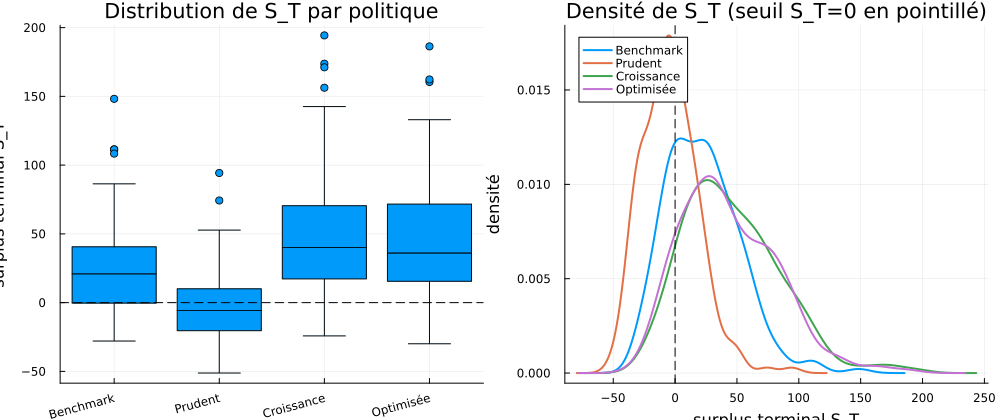
\includegraphics[width=\textwidth]{comparaison_benchmarks.png}
\caption{Distribution du surplus terminal $S_T$ par politique sur les $200$
trajectoires hors échantillon~: boîtes à moustaches (gauche) et densités
superposées (droite). Le trait pointillé marque le seuil de solvabilité
$S_T = 0$~; la masse à sa gauche est le sous-financement terminal, que la CSaR
pénalise.}
\label{fig:comparaison}
\end{figure}

Le tableau~\ref{tab:horsech} et la figure~\ref{fig:comparaison} appellent une
lecture en deux temps, dont le second est le plus instructif.

Premier temps~: contre les politiques modérées, la domination de la politique
optimisée est écrasante et porte précisément là où le modèle est censé agir.
Face au benchmark diversifié, elle double le surplus moyen ($43{,}6$ contre
$22{,}4$) tout en \emph{réduisant} la queue ($\CSaR$ de $-16{,}2$ contre
$-25{,}6$) et en abaissant le sous-financement, terminal ($11{,}5\,\%$ contre
$26{,}0\,\%$) comme de chemin ($35{,}0\,\%$ contre $48{,}5\,\%$). Le
portefeuille prudent, lui, illustre un point structurel du problème en
run-off~: avec un surplus moyen \emph{négatif} et trois trajectoires sur
quatre passant sous l'équilibre, la prudence d'allocation est ici la stratégie
la plus risquée qui soit --- privé de cotisations, un fonds qui ne prend pas de
risque d'actif est mécaniquement érodé par son décaissement. La solvabilité
d'un fonds fermé ne s'obtient pas en fuyant le risque, mais en le
dimensionnant.

Second temps, plus inconfortable et assumé comme tel~: face au portefeuille
croissance --- construit \emph{a posteriori} en copiant l'agressivité moyenne
de la solution optimale ---, la politique multi-étapes fait essentiellement
jeu égal ($\E[S_T]$ de $43{,}6$ contre $46{,}1$, CSaR et métriques de chemin
quasi identiques, léger avantage de chemin à l'optimisée). L'explication est
dans le tableau~\ref{tab:alloc}~: l'allocation optimale varie peu d'une
période à l'autre, car les bornes de placement saturées compriment l'espace où
le recours pourrait s'exprimer~; une politique fixe bien choisie en est alors
une excellente approximation. Deux réserves empêchent toutefois d'en conclure
que la flexibilité ne vaut rien. D'une part, le portefeuille croissance n'est
pas une politique disponible \emph{ex ante}~: il est calqué sur la solution du
modèle, qu'il faut avoir résolu pour le connaître --- c'est un adversaire
construit après coup, et le fait même qu'il soit dur à battre est une
validation de la décision moyenne du modèle plutôt qu'un désaveu du recours.
D'autre part, l'avantage résiduel de l'optimisée est concentré exactement où
la théorie le prédit~: sur la solvabilité de chemin ($35{,}0\,\%$ contre
$36{,}0\,\%$, et un $\min_t \mathrm{FR}_t$ moyen comparable), qu'elle seule
surveille explicitement via le ré-ancrage de $\delta$ à chaque date. Sur cette
fenêtre de calibration, la valeur de la flexibilité multi-étapes est donc
réelle mais modeste, et logée dans les queues et le chemin plutôt que dans la
moyenne~; la sensibilité aux drifts, ci-dessous, montrera que cette conclusion
est elle-même dépendante de la générosité de la fenêtre.

Reste la direction que l'évaluation précédente ne couvre pas~: le risque de
modèle. On y répond par un test de \emph{mauvaise spécification}~: $200$
nouvelles trajectoires (graine dédiée) sont simulées sous le drift sobre de
l'analyse~(a) --- $5\,\%$ log pour XIC et VFV, covariances inchangées ---
pendant que la politique optimisée \emph{conserve ses croyances de la
fenêtre}~: décision initiale du cas de base, sous-arbres construits avec les
drifts estimés, ré-ancrage de $\delta$ au plancher de chaque sous-arbre,
exactement comme ci-dessus. Le gestionnaire optimise donc sur un monde qui
n'est plus le vrai. Les $800$ sous-problèmes restent tous faisables ---
l'ancrage tient aussi hors de ses hypothèses.

\begin{table}[htbp]
\centering
\caption{Test de mauvaise spécification~: mêmes politiques, $200$ trajectoires
simulées sous drift sobre ($5\,\%$ log sur les actions), la politique
optimisée conservant les croyances de la fenêtre d'estimation. Mêmes colonnes
que le tableau~\ref{tab:horsech}.}
\label{tab:stress}
\begin{tabular}{lccccc}
\toprule
Politique & $\E[S_T]$ & $\CSaR_{0{,}95}$ & $\prob(S_T<0)$ &
$\prob(\min_t \mathrm{FR}_t < 1)$ & $\E[\min_t \mathrm{FR}_t]$ \\
\midrule
Benchmark diversifié & $-11{,}6$ & $-51{,}0$ & $74{,}5\,\%$ & $82{,}5\,\%$ & $0{,}882$ \\
Prudent              & $-18{,}0$ & $-56{,}0$ & $83{,}5\,\%$ & $90{,}0\,\%$ & $0{,}853$ \\
Croissance           & $-6{,}2$  & $-50{,}0$ & $63{,}0\,\%$ & $75{,}5\,\%$ & $0{,}899$ \\
Optimisée (multi-étapes) & $-7{,}0$ & $-50{,}5$ & $64{,}5\,\%$ & $77{,}0\,\%$ & $0{,}896$ \\
\bottomrule
\end{tabular}
\end{table}

Avant toute lecture fine, le rappel de précision s'impose~: à $200$
trajectoires, l'erreur type d'une proportion avoisine $3{,}5$ points, et les
écarts entre Croissance et Optimisée dans le tableau~\ref{tab:stress}
($1{,}5$ point de sous-financement, $0{,}8$ de surplus moyen) sont dans
l'épaisseur du trait. Trois constats robustes s'en dégagent néanmoins.
D'abord, le tableau est le pendant \emph{par trajectoires} de la
sensibilité~(a)~: sous croyances sobres, plus aucune politique ne protège ---
tous les surplus moyens sont négatifs, et le sous-financement terminal de la
politique optimisée passe de $11{,}5$ à $64{,}5\,\%$. La sécurité du
tableau~\ref{tab:horsech} était bien empruntée à la fenêtre, et aucun talent
d'allocation ne la restitue. Ensuite, la hiérarchie entre familles
persiste~: les politiques agressives (Croissance, Optimisée) dominent
nettement le benchmark et surtout le portefeuille prudent, qui reste le pire
des mondes ($83{,}5\,\%$ de sous-financement) --- même sous un drift sobre,
fuir le risque d'actif ne sauve pas un fonds fermé de son décaissement.
Enfin, et c'est le point propre à ce test~: la mauvaise spécification
n'inflige \emph{pas} de pénalité détectable à la politique optimisée
relativement à son homologue fixe --- optimiser sur de mauvaises croyances
n'a pas fait pire que de figer les poids, le coût étant porté par
l'exposition actions elle-même et non par le mécanisme de recours. C'est une
propriété rassurante du dispositif, mais qui doit être énoncée avec sa
précision~: au bruit d'échantillonnage près.

\subsection{Analyses économiques}\label{ssec:resultats-analyses}

Les analyses qui suivent déclinent la même question --- qu'est-ce qui, dans
les résultats du cas de base, est structurel, et qu'est-ce qui est emprunté à
la fenêtre d'estimation~? --- le long de sept axes. Le fil conducteur en est
le plancher $\taustar$ introduit en section~\ref{ssec:taustar}.

\paragraph{(a) Sensibilité aux rendements espérés~: ce que la fenêtre donne.}
La section~\ref{ssec:calibration} a établi que les drifts actions sont à la
fois décisifs et fragiles. On les remplace donc par un drift \emph{sobre} de
$5\,\%$ (log) pour XIC comme VFV --- ordre de grandeur d'une prime de risque
de long terme --- en conservant tout le reste, covariances comprises, et l'on
recalcule l'ensemble du cas de base~:

\begin{center}
\begin{tabular}{lcc}
\toprule
 & Base (fenêtre 2013--2026) & Drift sobre ($5\,\%$) \\
\midrule
$\E[S_T]$                 & $56{,}15$  & $10{,}60$ \\
$\CSaR_{0{,}95}(S_T)$     & $-14{,}43$ & $-38{,}92$ \\
$\prob(\mathrm{FR}_T<1)$  & $7{,}2\,\%$ & $40{,}1\,\%$ \\
$\taustar$                & $0{,}0108$ & $0{,}0423$ \\
\bottomrule
\end{tabular}
\end{center}

La lecture est sans ambiguïté~: sous croyances sobres, le surplus moyen fond
de $81\,\%$, la probabilité de sous-financement terminal est multipliée par
plus de cinq, et la solvabilité incompressible $\taustar$ par près de quatre.
La sécurité apparente du cas de base --- $7\,\%$ de sous-financement, queue
contenue --- est donc, pour l'essentiel, \emph{empruntée} au marché haussier
de la fenêtre d'estimation~: environ $33$ points de probabilité de
sous-financement ($40{,}1\,\%$ contre $7{,}2\,\%$) reposent sur la
persistance de drifts actions historiquement exceptionnels. C'est le résultat
que nous considérons comme le plus important de ce travail pour la pratique~:
aucune optimisation ne crée cette sécurité, elle ne fait que la transporter
depuis les hypothèses de rendement.

\paragraph{(b) Balayage de la tolérance~: la frontière de faisabilité.}
On fait varier $\delta$ autour du plancher, toutes choses égales par
ailleurs~:

\begin{center}
\begin{tabular}{cccccc}
\toprule
$\delta$ & $\delta/\taustar$ & Faisable & $\E[S_T]$ & $\CSaR$ & Duals ICC (somme) \\
\midrule
$0{,}0087$ & $0{,}80$ & non & --- & --- & --- \\
$0{,}0103$ & $0{,}95$ & non & --- & --- & --- \\
$0{,}0108$ (arrondi) & $0{,}997$ & non & --- & --- & --- \\
$\taustar$ (exact) & $1{,}00$ & oui & $55{,}81$ & $-14{,}39$ & $57{,}7$ \\
$0{,}0120$ & $1{,}11$ & oui & $56{,}15$ & $-14{,}43$ & $0$ \\
$0{,}0141$ & $1{,}30$ & oui & $56{,}15$ & $-14{,}43$ & $0$ \\
$0{,}0217$ & $2{,}00$ & oui & $56{,}15$ & $-14{,}43$ & $0$ \\
\bottomrule
\end{tabular}
\end{center}

Trois enseignements. D'abord la frontière est exactement où la théorie la
place~: infaisable strictement sous $\taustar$, faisable au plancher --- à
condition d'y prendre $\taustar$ \emph{exact}~: le point à $\delta =
\taustar$ arrondi au plus proche ($0{,}0108$, ratio $0{,}997$) est
infaisable, illustration numérique directe de la
remarque~\ref{rem:arrondi}, désormais lisible dans le tableau. Ensuite, les duals ne sont non nuls
que \emph{sur} la frontière ($57{,}7$ au total, sans valeur aberrante, avec un
coût visible~: $\E[S_T]$ y perd $0{,}34$)~; dès $1{,}10\,\taustar$ la
contrainte est lâche et la solution rejoint l'optimum libre. L'ICC de ce
problème n'est donc pas un prix marginal qui sculpte la solution à
l'intérieur du domaine, mais une \emph{contrainte de frontière}~: tout son
contenu économique est concentré dans le plancher $\taustar$ qu'elle induit.
Enfin, cette géométrie explique les duals nuls du cas de base sans les
excuser~: la marge de $10\,\%$ ne « fait rien » au cas de base, et l'on est en
droit de demander ce qu'elle achète --- c'est l'objet de l'analyse~(h).

\paragraph{(c) Capitalisation initiale~: la convexité du plancher.}
En faisant varier le ratio de capitalisation initial à passif donné, on
obtient $\taustar = 0{,}0402$ pour $\mathrm{FR}_0 = 0{,}9$, $0{,}0108$ pour
$\mathrm{FR}_0 = 1$ et $0{,}0022$ pour $\mathrm{FR}_0 = 1{,}1$, avec des
surplus moyens de $36{,}5$, $56{,}2$ et $75{,}8$ et des probabilités de
sous-financement de $16{,}5\,\%$, $7{,}2\,\%$ et $2{,}5\,\%$. Dix points de
capitalisation initiale déplacent donc la solvabilité incompressible de près
d'un facteur quatre dans chaque direction~: $\taustar$ est fortement convexe
en la dotation initiale, et un fonds fermé sous-doté part avec un handicap de
solvabilité qu'aucune allocation ne rattrape --- la version quantitative de
l'adage selon lequel, en run-off, tout se joue à la fermeture.

\paragraph{(d) Rythme de décaissement.}
Un profil de décaissement plat à $2\,\%$ ramène $\taustar$ à $0{,}0102$ et
porte $\E[S_T]$ à $63{,}2$ ($\prob(\mathrm{FR}_T<1) = 3{,}9\,\%$)~; un profil
accéléré de $3$ à $6\,\%$ pousse $\taustar$ à $0{,}0138$ et fait chuter
$\E[S_T]$ à $44{,}7$ ($12{,}9\,\%$). La pente des prestations agit ainsi sur
la solvabilité incompressible dans le même sens que la sous-capitalisation,
mais plus doucement~: le levier dominant reste $\mathrm{FR}_0$.

\paragraph{(e) Aversion au risque.}
Le long de la grille $\lambda \in \{0,\ 0{,}5,\ 1,\ 2,\ 5\}$, l'espérance du
surplus décroît de $56{,}6$ à $55{,}4$ pendant que la CSaR (recalculée ex post
pour $\lambda = 0$, conformément à la remarque~\ref{rem:lambda-zero})
s'améliore de $-16{,}4$ à $-14{,}1$~: la frontière espérance--CSaR est
étroite. La cause est la même que celle rencontrée à la
section~\ref{ssec:resultats-he}~: les bornes de placement mordent avant les
préférences, et l'allocation ne peut pas s'écarter beaucoup de son point de
saturation quelle que soit l'aversion. Seule la décision racine bouge
sensiblement (XIC passe de $30$ à $40\,\%$ entre $\lambda = 0$ et
$\lambda \ge 0{,}5$).

\paragraph{(f) Le recours en action.}
Aux n\oe uds de profondeur $t = 2$ ($50$ n\oe uds), la part actions de la
solution est corrélée positivement au ratio de capitalisation courant
($+0{,}24$) et la part d'or négativement ($-0{,}24$)~: par quartile de
$\mathrm{FR}$, la part actions passe de $68\,\%$ (quartile le plus pauvre,
$\mathrm{FR} \in [0{,}85, 1{,}08]$) à $77\,\%$ (le plus riche), l'or de
$5{,}4\,\%$ à $3{,}1\,\%$. Le modèle applique donc une gestion
\emph{procyclique} du surplus --- prendre du risque quand le coussin le
permet, se couvrir quand il s'amincit --- qui est la signature qualitative
attendue d'un recours rationnel sous contrainte de solvabilité~; son
amplitude, quelques points de pourcentage, est là encore bridée par les
bornes.

\paragraph{(g) Le prix de la cohérence temporelle.}
Le plancher conditionnel, calculé en transposant le minimax à l'écriture
n\oe ud par n\oe ud du modèle institutionnel (section~\ref{ssec:taustar}),
vaut $\taustar_{\mathrm{cond}} = 0{,}2139$, contre $\taustar = 0{,}0108$ en
écriture inconditionnelle --- un rapport de vingt. Exiger la tenue du seuil
dans \emph{chaque} état, et non en moyenne vue de la racine, est donc hors de
portée d'un fonds fermé~: il faudrait tolérer un manque espéré de plus de
$21\,\%$ du passif état par état pour que la contrainte conditionnelle soit
seulement réalisable. L'écart $\taustar_{\mathrm{cond}} - \taustar =
0{,}2030$ est la mesure, en points de passif, de ce que le fonds a perdu en
capacité de solvabilité en perdant ses cotisations~: c'est l'argument
économique le plus net de ce travail en faveur des mécanismes de redressement,
et la justification a posteriori du choix d'ICC inconditionnelles fait en
section~\ref{ssec:positionnement}.

\paragraph{(h) Utilité des ICC~: le budget de robustesse, et son étroitesse.}
Reste la question laissée ouverte par le balayage~(b)~: à quoi sert une marge
que le cas de base ne consomme pas~? On y répond en fixant $\delta = 0{,}0120$
--- sa valeur du cas de base --- et en faisant glisser les drifts actions de
leur valeur estimée ($\alpha = 1$) vers le drift sobre de $5\,\%$
($\alpha = 0$)~:

\begin{center}
\begin{tabular}{ccccc}
\toprule
$\alpha$ & $\hat\mu_{\mathrm{VFV}}$ & Manque libre max & $\taustar_\alpha$ &
$\delta = 0{,}0120$ faisable~? \\
\midrule
$1{,}00$ & $0{,}163$ & $0{,}0109$ & $0{,}0108$ & oui (duals nuls) \\
$0{,}95$ & $0{,}157$ & $0{,}0116$ & $0{,}0115$ & oui (duals nuls) \\
$0{,}90$ & $0{,}152$ & $0{,}0122$ & $0{,}0121$ & \textbf{non} \\
$0{,}80$ & $0{,}140$ & $0{,}0138$ & $0{,}0136$ & non \\
$0{,}60$ & $0{,}118$ & $0{,}0182$ & $0{,}0167$ & non \\
$0{,}00$ & $0{,}050$ & $0{,}0463$ & $0{,}0423$ & non \\
\bottomrule
\end{tabular}
\end{center}

Deux faits structurent ce tableau. D'abord, à chaque niveau de croyances, le
manque libre colle au plancher ($\taustar_\alpha$ à quelques $10^{-4}$
près)~: l'objectif CSaR est presque minimax en manque de chemin, et l'ICC ne
connaît pour ainsi dire que deux états --- dormante ou infaisable. La
transition se produit entre $\alpha = 0{,}95$ et $\alpha = 0{,}90$~: une
révision du drift VFV comprise entre $60$ et $110$ points de base --- bien
moins que l'erreur type d'estimation de ce même drift
(section~\ref{ssec:calibration}) --- suffit à rendre infaisable la tolérance
calibrée la veille. La marge de $10\,\%$ sur $\taustar$ est donc un
\emph{budget de robustesse aux croyances}, et il est étroit~: il n'absorbe
même pas une erreur d'estimation typique du paramètre le plus fragile du
modèle. La conséquence pratique est celle annoncée en
section~\ref{ssec:taustar}~: l'ancrage de $\delta$ sur un $\taustar$
\emph{recalculé avec les données} n'est pas une élégance méthodologique mais
une nécessité opérationnelle --- tout seuil figé, si raisonnable soit-il au
moment de sa fixation, a une espérance de vie qui se mesure en points de base
de drift. Et c'est le pendant, côté contraintes, de la sensibilité~(a)~: la
solvabilité apparente du fonds est empruntée à la fenêtre, et l'ICC ---
l'instrument qui la surveille --- est le premier composant du modèle à
encaisser la restitution de l'emprunt.

% ==================================================================
\section{Limites et extensions}\label{sec:limites}
% ==================================================================

Les limites de ce travail ont été signalées au fil du texte, à l'endroit où
chacune agit~; cette section les rassemble, les hiérarchise, et esquisse les
extensions qui les lèveraient.

\subsection{Limites}\label{ssec:limites-liste}

\emph{L'indépendance passif--rendements} ($g \perp r$) est la plus lourde. Elle
prive le modèle de toute notion d'appariement~: un passif dont la croissance ne
co-varie avec aucun actif ne peut être couvert par aucun, et la distinction
économique centrale entre obligations nominales et réelles devient invisible
--- XRB n'est plus, pour l'optimiseur, qu'une seconde ligne obligataire
corrélée à $0{,}87$ avec la première (tableau~\ref{tab:calib}), ce que la
substitution erratique XIC--XRB de l'étude inter-graines reflète directement.
Les résultats d'allocation entre lignes obligataires ne doivent donc pas être
interprétés.

\emph{La mesure de risque terminale est statique.} La CSaR porte sur $S_T$ vu
de la racine~; elle n'est pas temporellement cohérente au sens des mesures
imbriquées, et une politique optimale vue de $t=0$ peut cesser de l'être
conditionnellement à un état intermédiaire. Le contraste quantifié entre
$\taustar$ et $\taustar_{\mathrm{cond}}$ (analyse~(g)) montre précisément ce
que coûterait la version cohérente~: elle est hors de portée du fonds fermé,
et c'est bien pourquoi nous l'avons affaiblie --- mais le choix reste un
choix, et il est assumé.

\emph{Les log-rendements sont i.i.d.\ gaussiens.} Ni queues épaisses, ni
corrélations dépendant du régime, ni retour à la moyenne~: l'arbre hérite des
limites du GBM. Les queues de nos distributions terminales sont donc
vraisemblablement optimistes, et la CSaR sous-estimée en niveau --- mais les
\emph{comparaisons} entre politiques, toutes évaluées sous la même dynamique,
en souffrent moins.

\emph{Le décaissement est déterministe}, proportionnel au passif \emph{espéré}
plutôt qu'au passif réalisé~: les flux ne réagissent pas à l'état. C'est
cohérent avec des prestations définies contractuellement, mais cela neutralise
le canal par lequel un passif réalisé plus lourd exigerait des décaissements
plus lourds~; la sensibilité~(d) à la pente de $F_t$ donne l'ordre de grandeur
de ce qui se joue là.

\emph{L'horizon est court.} Cinq ans ne sont que la première tranche d'un
run-off qui s'étale sur des décennies~: conformément à la discussion de la
section~\ref{ssec:passif}, la croissance nette positive du passif cesse
d'être tenable au-delà, et $\taustar$ s'interprète comme la solvabilité
incompressible \emph{sur cette fenêtre}, non sur l'extinction complète. La
contrainte est technologique --- la taille de l'arbre croît
exponentiellement avec $T$ --- et son dépassement passe par la décomposition
évoquée en extension (SDDP, section~\ref{ssec:extensions}).

\emph{La fenêtre d'estimation est courte et haussière.} C'est la limite la
mieux quantifiée du document (analyses~(a) et~(h))~: l'essentiel de la
sécurité apparente du cas de base est emprunté aux drifts de la fenêtre, et le
dispositif de calibration lui-même ($\delta$ ancré à $\taustar$) ne survit
qu'à une révision de croyances inférieure à l'erreur type des drifts. Nous ne
le répétons pas davantage~; c'est le message central.

\emph{Divers.} La poche VFV est portée non couverte --- le risque de change
est modélisé implicitement via les rendements en dollars canadiens, avec le
pari de drift qu'assume et chiffre la section~\ref{ssec:univers}~; CGL reste
couvert par construction~;
la concentration effective actions se réduit au couple XIC--VFV corrélé à
$0{,}68$~; l'or est modélisé par son seul cours (pas de revenu)~; les frais de
transaction et le rééquilibrage infra-période sont ignorés~; et l'actif est
fermé par hypothèse --- le levier des cotisations, dont l'analyse~(g) chiffre
la valeur en creux, est absent par construction.

\subsection{Extensions}\label{ssec:extensions}

Quatre directions prolongent naturellement le prototype, par ordre croissant
d'ambition. \emph{Réintroduire les cotisations}~: un terme de cotisation avec
coût de niveau et de variabilité dans l'objectif ramène au modèle
institutionnel de~\cite{KHSV2010} et permettrait de tester la prédiction de
l'analyse~(g) --- avec redressement, l'écart conditionnel--inconditionnel doit
se refermer. \emph{Coupler taux et passif}~: faire dépendre $g$ d'un facteur
de taux commun aux rendements obligataires rendrait à XRB et XLB leurs rôles
distincts et ferait émerger l'appariement --- c'est l'extension au meilleur
rapport enseignement/effort. \emph{Enrichir la génération de scénarios}~:
bootstrap par blocs (queues et autocorrélations empiriques) ou appariement de
moments~\cite{HoylandWallace2001} (réduction de la variance inter-graines à
taille d'arbre donnée).
\emph{Cohérence temporelle}~: mesures de risque imbriquées et décomposition
par programmation dynamique duale stochastique
(SDDP,~\cite{PereiraPinto1991}), qui lèveraient à la
fois la staticité de la CSaR et la contrainte de taille des arbres --- au prix
d'un changement de technologie complet.

% ==================================================================
\section{Conclusion}\label{sec:conclusion}
% ==================================================================

La question posée en introduction était double~: quelle allocation dynamique
pour un fonds de pension fermé, et --- plus fondamentalement --- quel niveau de
solvabilité est-il seulement \emph{possible} de garantir quand l'allocation est
le dernier levier restant~? La formulation en programme de recours multi-étapes,
armée des deux instruments du chapitre~6 de~\cite{KHvdVR2020}, a permis de
donner à cette seconde question une réponse chiffrée, et c'est le plancher de
faisabilité $\taustar$ --- introduit comme un expédient de calibration, devenu
l'objet central du travail --- qui la porte.

Sur les données gelées au 30~juin~2026, la solvabilité incompressible du fonds
étudié vaut $\taustar = 1{,}08\,\%$ du passif par période~: aucune allocation
admissible ne fait mieux, et toute exigence plus stricte est infaisable ---
non pas coûteuse, infaisable. Sa variante conditionnelle, qui exigerait la
tenue du seuil état par état comme dans le modèle institutionnel
de~\cite{KHSV2010}, vaut $21{,}4\,\%$~: vingt fois plus. Cet écart est à nos
yeux le résultat le plus parlant du document~: il chiffre exactement ce que le
fonds a perdu en fermant --- la cohérence temporelle de sa solvabilité --- et,
en creux, ce que valent les cotisations de redressement qui la rendraient
atteignable. Le balayage de la tolérance a précisé la géométrie de l'ICC dans
ce problème~: contrainte de frontière plutôt que prix marginal, dormante à
l'intérieur du domaine et infaisable au-delà, elle concentre tout son contenu
économique dans le plancher qu'elle induit~; et l'analyse~(h) a montré que la
marge de $10\,\%$ dont nous l'assortissons est un budget de robustesse aux
croyances consommé par une révision de $60$ à $110$ points de base du drift
actions --- moins que l'erreur type de ce même drift. L'ancrage de $\delta$ à
un $\taustar$ recalculé avec les données n'est donc pas une élégance mais une
nécessité opérationnelle.

Sur l'allocation elle-même, deux messages. La valeur de la flexibilité
multi-étapes, évaluée hors échantillon contre des politiques à poids fixes,
est réelle mais modeste, et logée là où la théorie la place~: dans les queues
et la solvabilité de chemin, pas dans la moyenne --- les bornes de placement,
en comprimant l'espace du recours, font d'une politique fixe agressive une
excellente approximation de la politique optimale --- et le test de mauvaise
spécification ajoute que ce constat survit au changement de monde~: optimiser
sur des croyances devenues fausses n'a pas coûté plus cher, au bruit
d'échantillonnage près, que de figer les poids. À l'inverse, la prudence
d'allocation s'est révélée être, en run-off, la stratégie la plus dangereuse
de toutes~: privé de cotisations, un fonds qui ne prend pas de risque d'actif
est mécaniquement érodé par ses décaissements. Enfin, l'honnêteté oblige à
encadrer tous ces chiffres par la sensibilité aux rendements espérés~: sous un
drift actions sobre, la probabilité de sous-financement terminal passe de
$7{,}2$ à $40{,}1\,\%$ et $\taustar$ quadruple. Une part substantielle de la
sécurité apparente du fonds est empruntée à la fenêtre 2013--2026~; aucune
optimisation ne crée cette sécurité, elle ne fait que la transporter depuis
les hypothèses.

Les prolongements naturels sont ceux de la section~\ref{ssec:extensions}~:
réintroduire les cotisations pour vérifier que l'écart
conditionnel--inconditionnel se referme, coupler taux et passif pour rendre
son sens à l'appariement obligataire, enrichir la génération de scénarios, et
--- à plus long terme --- passer aux mesures de risque imbriquées. Le
prototype présenté ici aura alors joué son rôle~: montrer qu'avec deux
instruments linéaires bien choisis, l'ICC et la CSaR, la question « que peut
l'allocation seule~? » admet une réponse quantitative, reproductible, et
honnête sur ses propres limites.

% ==================================================================
\appendix
\section{Linéarisation de la CSaR}\label{app:csar}

Cette annexe détaille l'équivalence entre la forme variationnelle du
lemme~\ref{lem:csar-var} et sa linéarisation~\eqref{eq:csar-lp} sur support
fini, qui fonde l'insertion de la CSaR dans le programme linéaire.

Soit $S$ à support fini $\{S_n\}_{n \in \mathcal F}$ de probabilités $p_n$, et
$H(\eta) := \E[\pos{\eta - S}] = \sum_n p_n \pos{\eta - S_n}$ la fonction de
manque espéré. La fonction
$f(\eta) := \eta - H(\eta)/(1-\gamma)$ est concave et affine par morceaux, de
pente $1 - F(\eta)/(1-\gamma)$ entre les atomes, où
$F(\eta) = \sum_n p_n \mathbf 1\{S_n \le \eta\}$ est la fonction de
répartition~: la pente est positive tant que $F(\eta) < 1-\gamma$ et négative
dès que $F(\eta) > 1-\gamma$. Le maximum de $f$ est donc atteint au quantile
de niveau $1-\gamma$, c'est-à-dire au premier atome $\eta^\star$ tel que
$F(\eta^\star) \ge 1-\gamma$. En ce point, en notant
$q := 1-\gamma$ et en décomposant $H(\eta^\star) =
\sum_{S_n < \eta^\star} p_n (\eta^\star - S_n)$, un calcul direct donne
\[
f(\eta^\star)
= \frac{1}{q}\Big[\sum_{S_n < \eta^\star} p_n S_n
+ \big(q - F(\eta^\star{}^-)\big)\,\eta^\star\Big],
\]
c'est-à-dire exactement la moyenne de la pire masse $q$ de la distribution,
l'atome au quantile n'étant compté que pour la masse manquante
$q - F(\eta^\star{}^-)$~: c'est la définition de la CSaR sur distribution
discrète (complétion au prorata, définition~6.4.1 de~\cite{KHvdVR2020}, et
lemme~6.4.2 pour la forme variationnelle, énoncé dans le livre pour une
distribution continue et étendu ici au cas discret).

La linéarisation remplace $H(\eta)$ par $\sum_n p_n u_n$ sous les contraintes
$u_n \ge \eta - S_n$, $u_n \ge 0$. Pour tout $(\eta, u)$ admissible,
$\sum_n p_n u_n \ge H(\eta)$, donc la valeur du programme linéarisé minore
$f(\eta)$ en tout point et le maximum linéarisé minore $\CSaR_\gamma(S)$~;
réciproquement, le choix $u_n = \pos{\eta - S_n}$ est admissible et atteint
$f(\eta)$. Le maximum du programme linéarisé vaut donc exactement
$\CSaR_\gamma(S)$. Lorsque ce bloc est inséré, affecté d'un poids
$\lambda > 0$, dans l'objectif~\eqref{eq:objectif} --- où $S_n = A_n - L_n$
dépend des décisions ---, l'argument vaut à décisions fixées~: à l'optimum
global, le bloc $(\eta, u)$ réalise la CSaR du surplus induit par les
décisions optimales, ce que la vérification ex post du cas de base confirme
numériquement à $3{,}6 \times 10^{-14}$ près
(section~\ref{ssec:validation}). Si $\lambda = 0$, plus rien ne pousse le
bloc vers son maximum et la valeur lue n'a pas de sens
(remarque~\ref{rem:lambda-zero}).

\section{Tableaux complémentaires}\label{app:tableaux}

\paragraph{Profil de manque libre par période.}
Manque espéré relatif $\sum_{t(n)=t} p_n D_n / \E[L_t]$ de la solution sans
ICC (cas de base par ailleurs)~: $0{,}0071$ ($t=1$), $0{,}0109$ ($t=2$),
$0{,}0074$ ($t=3$), $0{,}0070$ ($t=4$). Le maximum, $0{,}0109$, atteint en
$t=2$, coïncide à l'arrondi près avec $\taustar = 0{,}0108$~: c'est le fait
« objectif quasi-minimax » commenté aux
sections~\ref{ssec:resultats-base} et~\ref{ssec:resultats-analyses}.

\paragraph{Balayage complet de la tolérance.}
Version complète du tableau de l'analyse~(b), avec la probabilité de
sous-financement terminal~:

\begin{center}
\begin{tabular}{ccccccc}
\toprule
$\delta$ & $\delta/\taustar$ & Faisable & $\E[S_T]$ & $\CSaR$ &
Duals (somme) & $\prob(\mathrm{FR}_T<1)$ \\
\midrule
$0{,}0087$ & $0{,}80$ & non & --- & --- & --- & --- \\
$0{,}0103$ & $0{,}95$ & non & --- & --- & --- & --- \\
$0{,}0108$ (arrondi) & $0{,}997$ & non & --- & --- & --- & --- \\
$0{,}01083$ & $1{,}00$ & oui & $55{,}81$ & $-14{,}39$ & $57{,}7$ & $7{,}4\,\%$ \\
$0{,}0120$ & $1{,}11$ & oui & $56{,}15$ & $-14{,}43$ & $0$ & $7{,}2\,\%$ \\
$0{,}0141$ & $1{,}30$ & oui & $56{,}15$ & $-14{,}43$ & $0$ & $7{,}2\,\%$ \\
$0{,}0174$ & $1{,}61$ & oui & $56{,}15$ & $-14{,}43$ & $0$ & $7{,}2\,\%$ \\
$0{,}0217$ & $2{,}00$ & oui & $56{,}15$ & $-14{,}43$ & $0$ & $7{,}2\,\%$ \\
\bottomrule
\end{tabular}
\end{center}

On notera que serrer la contrainte jusqu'au plancher ne réduit pas la
probabilité de sous-capitalisation terminale ($7{,}4$ contre $7{,}2\,\%$)~: l'ICC
contrôle le manque espéré de chemin, pas la fréquence des déficits terminaux
--- deux grandeurs voisines mais distinctes, et c'est la CSaR qui gouverne la
seconde.

\paragraph{Grille complète de l'analyse~(h).}
Drifts actions interpolés entre la fenêtre ($\alpha=1$) et le drift sobre de
$5\,\%$ ($\alpha=0$), $\delta$ fixé à $0{,}0120$~:

\begin{center}
\begin{tabular}{ccccccc}
\toprule
$\alpha$ & $\hat\mu_{\mathrm{XIC}}$ & $\hat\mu_{\mathrm{VFV}}$ &
Manque libre max & $\taustar_\alpha$ & Faisable & Duals (somme) \\
\midrule
$1{,}00$ & $0{,}106$ & $0{,}163$ & $0{,}0109$ & $0{,}0108$ & oui & $0$ \\
$0{,}95$ & $0{,}103$ & $0{,}157$ & $0{,}0116$ & $0{,}0115$ & oui & $0$ \\
$0{,}90$ & $0{,}100$ & $0{,}152$ & $0{,}0122$ & $0{,}0121$ & non & --- \\
$0{,}85$ & $0{,}097$ & $0{,}146$ & $0{,}0130$ & $0{,}0128$ & non & --- \\
$0{,}80$ & $0{,}095$ & $0{,}140$ & $0{,}0138$ & $0{,}0136$ & non & --- \\
$0{,}60$ & $0{,}083$ & $0{,}118$ & $0{,}0182$ & $0{,}0167$ & non & --- \\
$0{,}40$ & $0{,}072$ & $0{,}095$ & $0{,}0267$ & $0{,}0239$ & non & --- \\
$0{,}20$ & $0{,}061$ & $0{,}073$ & $0{,}0358$ & $0{,}0325$ & non & --- \\
$0{,}00$ & $0{,}050$ & $0{,}050$ & $0{,}0463$ & $0{,}0423$ & non & --- \\
\bottomrule
\end{tabular}
\end{center}

\section{Code}\label{app:code}

\begin{sloppypar}
L'intégralité du code est livrée dans le \emph{notebook} Julia
\texttt{alm\_pension\_phases\_1a6\_julia\_2.ipynb}, accompagné du cache
de données \texttt{prix\_ajustes\_cache.csv}, du cache du diagnostic de
change \texttt{prix\_vsp\_cache.csv} et de la figure
\texttt{comparaison\_benchmarks.png}.
\end{sloppypar}
\begin{sloppypar} C'est ce \emph{notebook}, exécuté de
bout en bout sur noyau vierge (« Run All », environ deux minutes), qui a
produit chaque chiffre, tableau et figure du présent document~; une
réexécution les reproduit à l'identique aux précisions affichées
(section~\ref{ssec:implementation-code}).
\end{sloppypar}

Le code s'organise en six phases~: (1)~configuration, téléchargement (ou
rechargement du cache) et calibration~; (2)~génération de l'arbre~;
(3)~programme linéaire --- les deux fonctions c\oe ur sont
\texttt{solve\_alm} (équivalent déterministe
\eqref{eq:objectif}--\eqref{eq:c-icc}, avec $\delta$ optionnel et décalage de
période pour les sous-arbres) et \texttt{min\_tau\_uniform} (minimax
\eqref{eq:taustar})~; (4)~validation (forme fermée $T=1$, stabilité
inter-graines)~; (5)~évaluation hors échantillon (simulation, déroulés à poids
fixes et optimisé avec ré-ancrage de $\delta$, assertion de faisabilité sur
les $800$ sous-problèmes, puis test de mauvaise spécification sous drift
sobre)~; (6)~analyses économiques (a)--(h). Les graines
sont fixées et documentées~: \texttt{SEED0} $= 20240601$ (arbre principal et
analyses), $777$ (validation $T=1$), \texttt{SEED0}$+1$ à $12$ (stabilité),
$999$ et \texttt{base\_seed} $= 5000$ (hors échantillon), $998$ (trajectoires
du test de mauvaise spécification, qui réutilise \texttt{base\_seed} $= 5000$
pour ses sous-arbres, comme l'évaluation principale). Pour re-télécharger
des données fraîches, supprimer le fichier cache~; les résultats changeront
alors avec les données, et $\delta$ suivra $\taustar$ par construction.

% ==================================================================
\begin{thebibliography}{99}

\bibitem{Artzner1999}
P.~Artzner, F.~Delbaen, J.-M. Eber et D.~Heath,
\og Coherent measures of risk \fg,
\emph{Mathematical Finance}, vol.~9, n\textsuperscript{o}~3, p.~203--228, 1999.

\bibitem{Broadbent2006}
J.~Broadbent, M.~Palumbo et E.~Woodman,
\og The shift from defined benefit to defined contribution pension plans ---
implications for asset allocation and risk management \fg,
document de travail, Committee on the Global Financial System, Banque des
règlements internationaux, 2006.

\bibitem{Dert1995}
C.~L. Dert,
\emph{Asset Liability Management for Pension Funds: A Multistage Chance
Constrained Programming Approach},
thèse de doctorat, Université Érasme, Rotterdam, 1995.

\bibitem{Drijver2005}
S.~J. Drijver,
\emph{Asset Liability Management for Pension Funds Using Multistage
Mixed-Integer Stochastic Programming},
thèse de doctorat, Université de Groningue, 2005.

\bibitem{HoylandWallace2001}
K.~Høyland et S.~W. Wallace,
\og Generating scenario trees for multistage decision problems \fg,
\emph{Management Science}, vol.~47, n\textsuperscript{o}~2, p.~295--307, 2001.

\bibitem{KH1986}
W.~K. Klein~Haneveld,
\emph{Duality in Stochastic Linear and Dynamic Programming},
Lecture Notes in Economics and Mathematical Systems, vol.~274,
Springer, Berlin, 1986.

\bibitem{KHSV2010}
W.~K. Klein~Haneveld, M.~H. Streutker et M.~H. van~der~Vlerk,
\og An ALM model for pension funds using integrated chance constraints \fg,
\emph{Annals of Operations Research}, vol.~177, p.~47--62, 2010.

\bibitem{KHvdVR2020}
W.~K. Klein~Haneveld, M.~H. van~der~Vlerk et W.~Romeijnders,
\emph{Stochastic Programming: Modeling Decision Problems Under Uncertainty},
Springer, Cham, 2020.

\bibitem{PereiraPinto1991}
M.~V.~F. Pereira et L.~M.~V.~G. Pinto,
\og Multi-stage stochastic optimization applied to energy planning \fg,
\emph{Mathematical Programming}, vol.~52, p.~359--375, 1991.

\bibitem{RU2000}
R.~T. Rockafellar et S.~Uryasev,
\og Optimization of conditional value-at-risk \fg,
\emph{Journal of Risk}, vol.~2, n\textsuperscript{o}~3, p.~21--41, 2000.

\bibitem{SharpeTint1990}
W.~F. Sharpe et L.~G. Tint,
\og Liabilities --- a new approach \fg,
\emph{Journal of Portfolio Management}, vol.~16, n\textsuperscript{o}~2,
p.~5--10, 1990.

\end{thebibliography}

\end{document}
